\documentclass[12pt]{report}

\usepackage{listings}
\usepackage{float}
\usepackage{booktabs}
\usepackage{amssymb}
\usepackage{subcaption}
\usepackage{tikz}
\usetikzlibrary{positioning}

\usepackage{../../stile_appunti}
\lstset{style=stile-listings}

\begin{document}
	
	\generaFrontespizio{Sistemi Operativi}{2026}{Gabriele Tolomei}{m}
	
	\chapter{Introduzione all'hardware dei calcolatori}
	
	Per comprendere appieno il ruolo dei sistemi operativi, è utile richiamare una celebre affermazione del matematico e informatico Richard Hamming:
	
	\begin{quote}
		\textit{«Lo scopo del calcolo è la comprensione, non i numeri.»}
		\hfill --- Richard Hamming
	\end{quote}
	
	In modo del tutto analogo, possiamo affermare che lo scopo primario di un \textbf{Sistema Operativo} è l'\textbf{astrazione}, e non la semplice gestione meccanica dell'hardware. 
	
	Tuttavia, per poter costruire astrazioni corrette, stabili ed efficaci, è indispensabile padroneggiare in primo luogo il funzionamento della macchina fisica sottostante. 
	
	\begin{osservazione}{Virtualizzazione dell'hardware}{}
		I buoni sistemi operativi si distinguono proprio per la loro capacità di \textbf{virtualizzare} con successo i diversi aspetti dell'architettura hardware, fornendo ai programmi applicativi un'interfaccia semplificata e indipendente dai dettagli implementativi del livello fisico.
	\end{osservazione}
	
	In questo capitolo introduttivo verranno dunque fornite delle basi riguardanti l'archittettura degli elaboratori, in quanto queste conoscenze sono essenziali e necessarie al fine di comprendere \textit{come} e \textit{dove} lavora il Sistema Operativo.
	In particolare verranno trattate:
	
	\begin{enumerate}
		\item \textbf{L'architettura di von Neumann}: la struttura e il layout generale dell'elaboratore.
		\item \textbf{La CPU}: l'organizzazione interna comprendente registri, ALU, pipeline e suddivisione in core.
		\item \textbf{La gerarchia di memoria}: le tecnologie SRAM/DRAM, il principio di località e la gestione delle memorie cache.
		\item \textbf{Il sistema di Input/Output (I/O)}: il ruolo dei controller, la gestione degli interrupt e il meccanismo DMA (\textit{Direct Memory Access}).
	\end{enumerate}
	
	\section{Lo spettro Hardware-Software}
	
	Per comprendere il ruolo di un sistema operativo, è fondamentale analizzare la sua collocazione all'interno della gerarchia che separa il software applicativo dall'hardware sottostante. Ci si chiede quindi: \textit{dove si posiziona esattamente il sistema operativo?}
	
	L'architettura del sistema può essere suddivisa in tre macro-aree di esecuzione: lo \textbf{User Space} (spazio utente), il \textbf{Kernel Space} (spazio kernel) e la \textbf{Physical Machine} (macchina fisica).
	
	\begin{tabella}{l C}
		\textbf{Livello dell'Architettura} & \textbf{Ambito di Esecuzione} \\
		Applicazioni (\textit{Python, Java, C++, Web}) & \textbf{User Space} \\
		Librerie di Sistema (\textit{libc}) & \textbf{User Space} \\
		Sistema Operativo (\textit{Kernel}) & \textbf{Kernel Space} \\
		Firmware / Device Driver & \textbf{Hardware / Low-Level Space} \\
		Hardware (\textit{CPU, RAM, Controller I/O}) & \textbf{Physical Machine} \\
	\end{tabella}
	
	Parleremo in modo più approfondito del kernel e delle componenti di un Sistema Operativo più avanti nel corso.
	Come possiamo però vedere, il sistema operativo agisce come un vero e proprio \textit{ponte} tra il livello logico (le applicazioni in esecuzione) e il livello fisico (gli effettivi componenti hardware).
	
	Le astrazioni software fornite dai sistemi operativi devono necessariamente rispettare i limiti fisici imposti dall'hardware sottostante. La progettazione del software di sistema non può prescindere da questi vincoli, tra i quali spiccano in particolare:
	
	\begin{description}
		\item [Divario di velocità (\textit{Speed gap}):] Le CPU operano a frequenze molto elevate, riuscendo ad eseguire le istruzioni in frazioni di nanosecondo. Al contrario, i tempi di accesso alla memoria principale (DRAM) si misurano nell'ordine delle decine di nanosecondi. Questa marcata differenza prestazionale rende la memoria un frequente collo di bottiglia durante l'esecuzione dei processi.
		
		\item [Compromesso sulla memorizzazione (\textit{Storage trade-off}):] Esiste un vincolo fisico ed economico inscindibile tra velocità, capacità e costo della memoria. I dispositivi di storage più veloci (come le cache) sono estremamente costosi e di piccole dimensioni, mentre le memorie più economiche (come i dischi secondari) garantiscono capacità enormi ma a fronte di velocità decisamente inferiori.
		
		\item [Concorrenza (\textit{Concurrency}):] L'esecuzione parallela nei reali sistemi multi-core richiede un supporto hardware esplicito e dedicato per la sincronizzazione (ad esempio tramite istruzioni atomiche), indispensabile per evitare race condition e garantire la coerenza dei dati.
	\end{description}
	
	\begin{osservazione}{Ruolo del Sistema Operativo}{}
		Uno degli scopi primari nella progettazione degli algoritmi di un sistema operativo è proprio quello di mascherare ed erodere questi limiti fisici, offrendo ai programmi un'astrazione dell'hardware efficiente, omogenea e trasparente.
	\end{osservazione}
	
	\section{L'architettura di von Neumann (1945)}
	
	L'architettura di von Neumann rappresenta il fondamento teorico di quasi tutti i moderni calcolatori d'uso generale (\textit{general-purpose}).
	
	Tale modello si basa su due concetti chiave:
	\begin{description}
		\item [Concetto di programma memorizzato (\textit{Stored-Program}):] Le istruzioni e i dati condividono lo stesso spazio di memoria fisica (memorizzati in una memoria detta \textit{Memoria Centrale}).
		\item [Esecuzione sequenziale:] Le istruzioni vengono prelevate ed estratte una alla volta dalla memoria ed eseguite sequenzialmente dalla CPU. Non è previsto alcun tipo di concorrenza da questa architettura.
	\end{description}
	
	Di seguito forniamo uno schema grafico rappresentante la struttura del modello:
	
	\begin{center}
		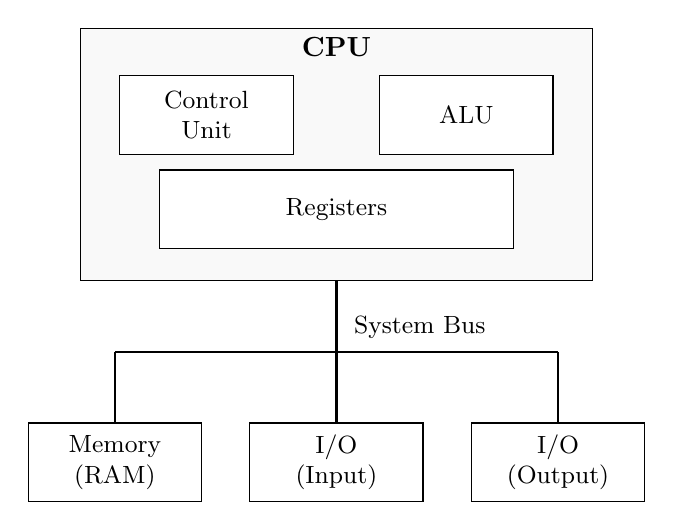
\begin{tikzpicture}[
			node distance=1.5cm,
			block/.style={draw, rectangle, minimum width=2.2cm, minimum height=1cm, align=center, fill=white, font=\small},
			cpu_box/.style={draw, rectangle, minimum width=6.5cm, minimum height=3.2cm, fill=gray!5},
			bus_line/.style={thick}
			]
			
			% CPU Box
			\node[cpu_box] (cpu) {};
			\node[anchor=north, font=\bfseries] at (cpu.north) {CPU};
			
			% Sub-components inside CPU
			\node[block, anchor=north west] (cu) at ([shift={(0.5cm,-0.6cm)}]cpu.north west) {Control\\Unit};
			\node[block, anchor=north east] (alu) at ([shift={(-0.5cm,-0.6cm)}]cpu.north east) {ALU};
			\node[block, minimum width=4.5cm, anchor=south] (reg) at ([shift={(0cm,0.4cm)}]cpu.south) {Registers};
			
			% Lower Blocks (posizionati sotto il bordo inferiore della CPU)
			\node[block, below=1.8cm of cpu.south] (io_in) {I/O\\(Input)};
			\node[block, left=0.6cm of io_in] (ram) {Memory\\(RAM)};
			\node[block, right=0.6cm of io_in] (io_out) {I/O\\(Output)};
			
			% Bus Split coordinate (a meta strada tra CPU e blocchi inferiori)
			\coordinate (bus_split) at ([yshift=-0.9cm]cpu.south);
			
			% Bus Connections
			\draw[bus_line] (cpu.south) -- (bus_split);
			\draw[bus_line] (ram.north |- bus_split) -- (io_out.north |- bus_split);
			
			\draw[bus_line] (ram.north) -- (ram.north |- bus_split);
			\draw[bus_line] (io_in.north) -- (bus_split);
			\draw[bus_line] (io_out.north) -- (io_out.north |- bus_split);
			
			% Bus Label (posizionato leggermente a lato dell'asta centrale per non sovrapporsi)
			\node[above right=0.05cm and 0.1cm of bus_split, font=\small] {System Bus};
			
		\end{tikzpicture}
	\end{center}
	
	L'architettura si articola nei seguenti elementi funzionali:
	
	\begin{description}
		\item [Unità Centrale di Elaborazione (CPU):] È il «cervello» del calcolatore, responsabile del coordinamento e dell'esecuzione di tutte le istruzioni. Al suo interno comprende:
		\begin{itemize}
			\item \textbf{Control Unit (Unità di Controllo):} Preleva le istruzioni dalla memoria, le decodifica e genera i segnali di controllo necessari al loro completamento.
			\item \textbf{ALU (Arithmetic Logic Unit):} Esegue le operazioni aritmetiche di base e le operazioni logiche elementari sui dati.
			\item \textbf{Registers (Registri):} Celle di memoria ad altissima velocità situate all'interno della CPU, impiegate per contenere temporaneamente dati, indirizzi di memoria o stati di esecuzione. Tra questi registri abbiamo, ad esempio:
			\begin{itemize}
				\item \textbf{Program Counter (PC)}, che si occupa di memorizzare l'indirizzo della prossima istruzione che deve essere eseguita dalla CPU.
				\item \textbf{Instruction Register (IR)}, che contiene il codice binario dell'effettiva istruzione puntata dal Program Counter.
			\end{itemize}
		\end{itemize}
		
		\item [Bus di Sistema (\textit{System Bus}):] È la struttura di collegamento condivisa (costituita da linee elettriche) attraverso la quale la CPU scambia indirizzi, dati e segnali di controllo con la memoria e le periferiche.
		
		\item [Memoria Principale (RAM):] Contiene sia il codice dei programmi in esecuzione sia i dati necessari al funzionamento delle applicazioni. Nel modello di von Neumann, istruzioni e dati condividono lo stesso spazio di memoria ed i medesimi bus.
		
		\item [Interfacce di I/O (Input/Output):] Moduli necessari a permettere l'interazione tra l'elaboratore e il mondo esterno, distinti in dispositivi di ingresso (\textit{Input}, come tastiera e mouse) e di uscita (\textit{Output}, come monitor e stampanti).
	\end{description}
	
	Tuttavia, come visto in precedenza, il principale svantaggio dell'architettura di von Neumann è proprio il fatto che le istruzioni e i dati condividono lo stesso spazio di memoria. Da ciò si origina il cosiddetto \textit{von Neumann Bottleneck}, cioè un effettivo limite fisico in quanto una memoria non può essere acceduta da più dispositivi contemporaneamente. Un'alternativa a questo modello è infatti il cosiddetto \textbf{Modello Harvard}, che prevede spazi di memoria e bus fisicamente separati per istruzioni e dati.
	
	\subsection{Il Bus di Sistema}
	Entriamo più nel dettaglio riguardo ai bus di sistema, che hanno l'importante compito di traspostare qualsiasi tipo di dato tra una componente e l'altra.
	
	\begin{description}
		\item [Bus Indirizzi (\textit{Address Bus}):] trasporta gli indirizzi di memoria dalla CPU verso i componenti di destinazione.
		Questo bus è \textbf{unidirezionale}, in quanto solo la CPU deve poter inviare l'indirizzo di memoria su cui lavorare.
		Inoltre, l'Address Bus ha una proprietà detta \textbf{Bus Width} (che fisicamente rappresenta quanti fili elettrici ci sono per quel bus) e che determina qual è il massimo numero di locazioni indirizzabili. La formula è molto semplice: se abbiamo $\text{width}=N$, il numero di locazioni indirizzabili è pari a $2^N$.
		
		\item [Bus Dati (\textit{Data Bus}):] gestisce il trasferimento dei byte di dati effettivi tra i vari componenti. Rappresenta il canale sul quale viaggia fisicamente l'istruzione da eseguire oppure il dato da elaborare. Poiché i dati devono poter essere scritti e letti, la trasmissione lungo il Data Bus è di tipo \textit{bidirezionale}. Anche questo bus possiede la proprietà di \textbf{Bus Width}, con significato analogo a quella dell'Address Bus, e questo valore in genere coincide con la Word Size del processore (dunque più è ampio il bus, maggiore è la quantità di dati che possono essere trasmessi simultaneamente).
		
		\item [Bus di Controllo (\textit{Control Bus}):] veicola i segnali di comando e di sincronizzazione del sistema, come le operazioni di lettura (\textit{read}), scrittura (\textit{write}), segnali di \textit{reset} o richieste di \textit{interrupt}. In sostanza, è il mezzo tramite cui la Control Unit (CU) definisce cosa fare con il dato e l'indirizzo selezionati.
	\end{description}
	
	\subsection{Il ciclo di istruzione}
	
	Il \textbf{ciclo di istruzione} (o \textit{fetch-decode-execute cycle}) rappresenta il processo fondamentale alla base del funzionamento di qualsiasi elaboratore. Ogni programma esegue questo ciclo in maniera continua.
	
	\begin{center}
		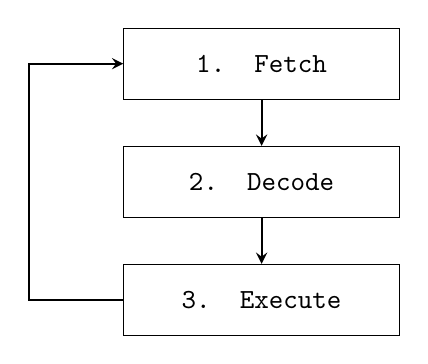
\begin{tikzpicture}[
			node distance=1.5cm,
			box/.style={draw, rectangle, minimum width=3.5cm, minimum height=0.9cm, align=center, font=\ttfamily\bfseries},
			arrow/.style={->, >=stealth, thick}
			]
			% Nodi
			\node[box] (fetch) {1. Fetch};
			\node[box, below of=fetch] (decode) {2. Decode};
			\node[box, below of=decode] (execute) {3. Execute};
			
			% Frecce principali
			\draw[arrow] (fetch) -- (decode);
			\draw[arrow] (decode) -- (execute);
			
			% Ciclo di ritorno
			\draw[arrow] (execute.west) -- ++(-1.2,0) |- (fetch.west);
		\end{tikzpicture}
	\end{center}
	
	Il ciclo si compone di tre fasi sequenziali gestite direttamente dalla CPU:
	
	\begin{enumerate}
		\item \textbf{Fetch (Prelevamento):} il contenuto del PC viene trasferito sull'Address Bus per poi prelevare l'effettiva istruzione puntata da quell'indirizzo. Alla fine di questa fase il valore del PC viene incrementato in modo di far passare all'istruzione successiva.
		
		\item \textbf{Decode (Decodifica):} il processore analizza e interpreta il significato della sequenza di bit che compone l'istruzione. Questa operazione viene svolta in base alla specifica codifica scelta dall'architettura dell'elaboratore (ossia l'\textit{Instruction Set Architecture} o ISA).
		
		\item \textbf{Execute (Esecuzione):} viene svolta l'operazione richiesta dall'istruzione. Questa fase può comportare un calcolo eseguito dall'Unità Aritmetico-Logica (ALU) oppure un'operazione di lettura/scrittura in memoria.
	\end{enumerate}
	
	Al termine della fase di esecuzione, il ciclo riparte immediatamente dalla fase di \textit{fetch} per l'istruzione successiva.
	
	\subsection{L'Unità Centrale di Elaborazione (CPU)}
	
	La \textbf{Central Processing Unit} (\textbf{CPU}) rappresenta il "cervello" del calcolatore, essendo l'organo fondamentale preposto all'esecuzione delle istruzioni memorizzate in memoria.
	
	L'architettura interna della CPU si articola su tre elementi costruttivi principali:
	
	\begin{enumerate}
		\item \textbf{Datapath (Unità Dati):} include l'\textbf{Arithmetic Logic Unit} (\textbf{ALU}), preposti alla manipolazione e al calcolo effettivo sui dati e i registri General-Purpose (adibiti al contenimento di risultati intermedi per le operazioni della ALU).
		
		\item \textbf{Control Unit} (\textbf{CU}): opera come coordinatore dell'intero microprocessore. Il suo compito è prelevare le istruzioni dalla memoria (\textit{fetch}), decodificarle e pilotare opportunamente il datapath per consentirne l'esecuzione.
		
		\item \textbf{Bus Interno:} insieme di canali e linee di interconnessione interne che mettono in comunicazione diretta i registri, l'ALU e la Control Unit.
	\end{enumerate}
	
	\subsection{Registri della CPU}
	Vediamo ora una carrellata veloce dei registri di sistema e delle loro funzionalità:
	
	\begin{enumerate}
		\item \textbf{Registri visibili all'utente (General-Purpose):} sono direttamente indirizzabili dalle istruzioni in linguaggio assembly per la manipolazione dei dati e l'esecuzione delle operazioni.
		
		\item \textbf{Registri di controllo e di stato (Special-Purpose):} sono utilizzati dalla \textit{Control Unit} (CU) per gestire lo stato di esecuzione del sistema e del processore. Tra i più rilevanti rientrano:
		\begin{itemize}
			\item \textbf{Program Counter (PC):} mantiene l'indirizzo della prossima istruzione da eseguire.
			
			\item \textbf{Instruction Register (IR):} contiene l'istruzione attualmente in fase di decodifica o esecuzione.
			
			\item \textbf{Processor Status Register (PSR):} memorizza le informazioni sullo stato corrente del processore (flag di condizione, livello di privilegio, ecc.).
			
			\item \textbf{Stack Pointer (SP):} contiene l'indirizzo di memoria della cima dello stack delle chiamate (ad esempio di chiamate delle funzioni).
			
			\item \textbf{Memory Address Register (MAR):} contiene l'indirizzo che sta per essere utilizzato dalla RAM. E' direttamente collegato all'Address Bus.
			
			\item \textbf{Memory Data Register (MDR):} contiene i byte di dati letti dalla RAM, ed è direttamente collegato al Data Bus.
			
		\end{itemize}
	\end{enumerate}
	
	\section{Pipelining delle istruzioni}
	
	Nei processori più semplici, il ciclo di esecuzione delle istruzioni segue un approccio strettamente sequenziale. Come previsto dal modello classico dell'architettura di Von Neumann, il processo avviene in modo sequenziale: la CPU deve completare interamente le fasi di prelievo (\textit{fetch}), decodifica (\textit{decode}) ed esecuzione (\textit{execute}) di una singola istruzione prima di poter passare a quella successiva. Questo schema, pur essendo semplice, comporta un notevole spreco di risorse hardware, poiché molte unità funzionali della CPU rimangono inattive durante le fasi in cui non sono direttamente coinvolte.
	
	Per superare questa limitazione e migliorare le prestazioni del sistema, si introduce una tecnica di ottimizzazione fondamentale:
	
	\begin{definizione}{Pipelining}{}
	Il \textbf{pipelining} è una tecnica di ottimizzazione hardware che consente di sovrapporre l'esecuzione di più istruzioni nel tempo, parallelizzando le diverse fasi del loro ciclo di vita.
	\end{definizione}
	
	Tale tecnica, almeno per le architetture di tipo RISC, si articola in 5 stadi:
	
	\begin{enumerate}
		\item \textbf{IF (Instruction Fetch):} prelievo dell'istruzione dalla cache di primo livello (L1 Cache) o dalla memoria principale (RAM).
		
		\item \textbf{ID (Instruction Decode):} decodifica dell'istruzione appena prelevata e lettura dei registri sorgente.
		
		\item \textbf{EX (Execute):} esecuzione del calcolo tramite l'unità aritmetico-logica (ALU) o calcolo dell'indirizzo di memoria.
		
		\item \textbf{MEM (Memory Access):} accesso alla memoria dati, che comporta un'operazione di lettura o scrittura verso la cache dati.
		
		\item \textbf{WB (Writeback):} scrittura del risultato finale all'interno del registro di destinazione.
	\end{enumerate}
	
	Grazie a questa suddivisione, ogni stadio opera su un'istruzione differente in modo simultaneo durante ciascun ciclo di clock, consentendo un'elevata sovrapposizione delle operazioni e migliorando l'efficienza del processore.
	
	\subsection{Hazard della pipeline}
	
	In condizioni ideali, le architetture con pipeline consentono di raggiungere il massimo incremento prestazionale. Tuttavia, nella realtà possono verificarsi delle situazioni anomale note come \textbf{hazard} (o criticità), che impediscono all'istruzione successiva di essere eseguita nel ciclo di clock prestabilito. 
	
	Tali criticità si dividono principalmente in tre grandi categorie:
	
	\begin{description}
		\item [Hazard strutturali (\textit{Structural Hazards}):] Si verificano in presenza di un conflitto di risorse, ovvero quando due o più stadi della pipeline richiedono contemporaneamente l'accesso allo stesso componente hardware fisico.
		
		\item [Hazard sui dati (\textit{Data Hazards}):] Si manifestano quando un'istruzione dipende strettamente dal risultato di un'istruzione precedente che non ha ancora completato il suo percorso all'interno della pipeline.
		
		\item [Hazard di controllo (\textit{Control Hazards}):] Sono causati dalle istruzioni di salto condizionato o incondizionato (\textit{branch}), le quali modificano il valore del \textit{Program Counter} (PC). Ciò rende invalide le istruzioni che sono già state caricate (\textit{fetched}) preventivamente nella pipeline.
		
	\end{description}
	
	Per risolvere tali criticità, le CPU moderne impiegano dei predittori di salto (\textbf{branch predictors}) per indovinare l'esito di un'istruzione di salto prima che essa venga effettivamente completata. Tuttavia, tali metodologie non verranno trattate.
	
	\section{Instruction Set Architectures (ISA)}
	\label{sec:instruction_set_architecture}
	
	Nel mondo dell'informatica sono stabiliti due standard principali riguardo al linguaggio adottato dalle istruzioni macchina:
	
	\begin{description}
		
		\item [CISC (Complex Instruction Set Computer):] ogni istruzione macchina può comprenderne altre (sono infatti a lunghezza variabile), in modo da "semplificare" la scrittura del software per gli utenti.
		
		\item [RISC (Reduced Instruction Set Computer):] mantiene solo le istruzioni principali del codice macchina (tutte hanno la stessa lunghezza).
		
	\end{description}
	
	\section{Processori Multi-Core}
	Gli elaboratori di oggi aggirano i limiti di potenza e velocità dei processori collocando più processori (detti appunto \textit{core}) su un singolo macro-processore.
	La caratteristica principale è proprio che ogni \textit{core} è come se fosse "autonomo", in quanto possiede i suoi registri e le sue unità di controllo.
	A questo punto deve essere il Sistema Operativo a saper gestire l'architettura Multi-Core: deve saper far comunicare efficientemente i vari core per la condivisione di risorse senza che si verifichino problemi di sincronizzazione delle variabili.
	Discuteremo di queste tecniche quando parleremo di \textit{concorrenza} e \textit{multi-threading}.
	
	\subsection{Prestazioni della CPU: Velocità di Clock e Cicli}
	
	Il funzionamento della CPU è sincronizzato da un \textbf{clock di sistema} ($System Clock$) oscillante, che scandisce il ritmo delle operazioni eseguite dal processore. Per comprendere le prestazioni di una CPU, è fondamentale analizzare due grandezze fondamentali legate a questo segnale:
	
	\begin{itemize}
		
		\item \textbf{Periodo di clock ($T$):} rappresenta la durata temporale di un singolo ciclo di clock (ad esempio $0.25$ nanosecondi).
		
		\item \textbf{Frequenza di clock ($f$):} rappresenta il numero di cicli di clock al secondo, misurata in Hertz ($\text{Hz}$).
		
	\end{itemize}
	
	Queste due grandezze sono inversamente proporzionali tra loro e legate dalla relazione:
	\[
	f = \frac{1}{T}
	\]
	
	A titolo d'esempio, una CPU a $4.0\text{ GHz}$ è in grado di completare $4 \times 10^9$ cicli di clock in un solo secondo.
	
	Tuttavia, non tutte le istruzioni macchina richiedono lo stesso tempo per essere eseguite: le istruzioni più semplici possono essere completate in un solo ciclo di clock, mentre le operazioni più complesse (come la divisione tra numeri in virgola mobile o gli accessi alla memoria principale) richiedono un numero elevato di cicli per poter essere portate a termine.
	
	Per valutare e confrontare l'efficienza dei processori, risulta fondamentale definire delle metriche standard. Una delle domande chiave nell'architettura dei calcolatori è: quante istruzioni riesce ad eseguire una CPU per ogni ciclo di clock? Per rispondere a questo interrogativo, introduciamo due parametri fondamentali:
	
	\begin{itemize}
		\item \textbf{CPI (Cycles Per Instruction):} rappresenta il numero medio di cicli di clock necessari per eseguire una singola istruzione.
		\item \textbf{IPC (Instructions Per Cycle):} rappresenta l'inverso del CPI, ovvero il numero di istruzioni eseguite in un singolo ciclo di clock. La relazione matematica è la seguente:
		\[
		\text{IPC} = \frac{1}{\text{CPI}}
		\]
	\end{itemize}
	
	Per calcolare il tempo totale necessario per eseguire un determinato programma, si utilizza la formula fondamentale delle prestazioni della CPU, che mette in relazione il numero di istruzioni, l'efficienza architetturale e la frequenza di clock:
	\[
	\text{CPU Time} = \text{Instruction Count} \times \text{CPI} \times \text{Clock Cycle Time}
	\]
	Dove con \textit{CPU Time} si intende il tempo totale necessario per eseguire tutte le istruzioni del programma. Analizzando i singoli componenti della formula:
	\begin{itemize}
		\item \textbf{Instruction Count:} il numero totale di istruzioni eseguite dal programma.
		\item \textbf{CPI:} il numero medio di cicli per istruzione.
		\item \textbf{Clock Cycle Time:} la durata di un singolo ciclo di clock (l'inverso della frequenza di clock).
	\end{itemize}
	
	\newpage
	\section{La gerarchia di memoria}
	La velocità dei processori, nel corso degli ultimi anni, è cresciuta molto più velocemente (si potrebbe dire in maniera quasi esponenziale) rispetto alla velocità di accesso alle memorie RAM. 
	Per continuare a velocizzare l'accesso alle risorse, gli architetti dei computer fanno riferimento ad una \textit{gerarchia delle memorie}, una struttura piramidale che organizza le memorie dall'alto verso il basso, dove quella più in \textbf{cima} sono i \textbf{registri}, memorie \textit{estremamente veloci}, situate all'interno della CPU, ma altrettanto costose; alla base di questa piramide si collocano i dispositivi di archiviazione di massa, come \textit{SSD} e \textit{HDD}, che sono più economiche ma decisamente più lente.
	Dunque, il compito di un bravo architetto di computer è quello di trovare il giusto compromesso a livello di prezzo e velocità, e il compito di un buon sistema operativo è quello di saper sfruttare queste risorse nel modo più efficiente possibile.
	
	Possiamo riassumere il comportamento della struttura con una regola fondamentale: \textbf{scendendo nella gerarchia, la velocità di accesso diminuisce, la capacità aumenta e il costo per byte diminuisce}.
	
	\begin{tabella}{|c|c|c|c|}
		\textbf{Livello} & \textbf{Componente} & \textbf{Capacità tipica} & \textbf{Latenza di accesso} \\
		L0 & CPU Registers & $< 1$ KiB & $< 0.5$ ns \\
		L1 & L1 Cache (per core) & $32 - 64$ KiB & $1 - 2$ ns \\
		L2 & L2 Cache (per core) & $256 - 512$ KiB & $3 - 5$ ns \\
		L3 & L3 Cache (shared) & $8 - 64$ MiB & $10 - 20$ ns \\
		L4 & Main Memory (DRAM) & $8 - 64$ GiB & $60 - 100$ ns \\
		L5 & SSD (NAND Flash) & $256$ GiB - $2$ TiB & $10 - 100$ $\mu$s \\
		L6 & HDD (Magnetic Disk) & $1 - 10$ TiB & $5 - 10$ ms \\
	\end{tabella}
	
	\newpage
	La memoria principale è strutturata come una griglia monodimensionale di indirizzi di byte (\textit{byte addresses}). Ogni cella possiede un indirizzo univoco a cui corrisponde un determinato contenuto memorizzato.
	
	\subsection{Il principio di località}
	
	L'efficacia della gerarchia di memoria (\textit{memory hierarchy}) si basa sul "principio di località", che definisce una serie di principi secondo i quali lavora la CPU per ottimizzare l'accesso alle informazioni. I programmi in esecuzione non accedono infatti alla memoria in modo casuale, ma presentano due forme fondamentali di località:
	
	\begin{description}
		\item [\textbf{Località temporale (\textit{Temporal Locality}):}] se una determinata locazione di memoria viene acceduta una volta, è molto probabile che la stessa locazione venga acceduta nuovamente nel futuro prossimo. Ad esempio, in un ciclo \texttt{for} in cui si accede alla variabile \texttt{i} per ogni iterazione del ciclo, la CPU dovrà accedere sempre alle stesse variabili e dunque terrà memorizzato in qualche registro vicino alla CPU l'indirizzo di memoria di quelle variabili.
		
		\item [\textbf{Località spaziale (\textit{Spatial Locality}):}] se viene acceduta una specifica locazione di memoria, è molto probabile che anche le locazioni ad essa vicine o adiacenti vengano accedute nel prossimo futuro. Tenendo sempre l'esempio del ciclo \texttt{for}, vedendo che tali locazioni di memoria vengono usate spesso, la CPU tende a memorizzare quei valori nei registri più vicini ad essa, in modo da renderne l'accesso quasi immediato.
	\end{description}
	
	\subsection{Architettura della Cache Memory}
	
	Le memorie cache non gestiscono i dati a livello di singoli byte, ma operano su blocchi di dimensione fissa denominati \textbf{cache line} (la cui dimensione tipica è di $64\text{ byte}$).
	
	Ogni entry all'interno di una cache line è composta da tre elementi fondamentali:
	\begin{description}
		\item[Valid Bit:] Un bit di controllo che indica se i dati presenti nella linea di cache sono validi ed aggiornati. Questo flag permette di verificare se il dato cercato è effettivamente presente ed utilizzabile all'interno della cache.
		\item[Tag Bit:] Identifica l'indirizzo di memoria originale (in RAM) da cui sono stati reperiti i dati. Agisce in modo analogo alla chiave di un dizionario: permette di stabilire in modo univoco a quale posizione della memoria principale appartenga il blocco.
		\item[Data Block:] Contiene l'effettivo blocco di dati copiato dalla memoria RAM (tipicamente $64\text{ byte}$), ovvero il contenuto informativo richiesto situato a quell'indirizzo.
	\end{description}
	
	Nel momento in cui la CPU richiede un determinato indirizzo di memoria (\textit{memory address}), si possono verificare due situazioni distinte:
	
	\begin{description}
		
		\item [Cache Hit (Dato trovato)] Si ha un \textit{cache hit} quando la CPU individua con successo l'indirizzo e il dato cercato direttamente all'interno della memoria cache.
		
		\item [Cache Miss (Dato non trovato)] Si ha un \textit{cache miss} quando la CPU non trova l'indirizzo richiesto all'interno della memoria cache, rendendo necessario il recupero del dato da memorie più lente.
		
	\end{description}
	
	\subsection{Politiche di scrittura della Cache}
	Nel momento in cui la CPU scrive i dati in un cache block, possono essere applicate due politiche per mantenere aggiornata la RAM:
	\begin{description}
		\item [Write-Through:] la CPU scrive contemporaneamente sia nella cache che nella memoria centrale. Il vantaggio è ovviamente una sincronizzazione costante dei dati; lo svantaggio è che una semplice operazione di scrittura di un dato sarà sempre lenta in quanto si dovrà riportare anche in memoria centrale, e dunque elimina il vantaggio di utilizzo della cache.
		
		\item [Write-Back:] la CPU scrive solo nella cache line e la marca come "modificata". L'aggiornamento effettivo nella memoria centrale si verifica solo quando tale cache line viene espulsa dalla cache per fare spazio ad altri dati. Vantaggioso in quanto viene mantenuta la velocità di memorizzazione di dati all'interno della cache, ma rimane il problema possibile della sincronizzazione.
	\end{description}
	
	\subsection{Politiche di mapping della Cache Line}
	
	Una questione fondamentale nell'organizzazione delle architetture dei calcolatori riguarda il criterio secondo cui un blocco della memoria principale (\textit{memory block}) viene posizionato all'interno di uno slot della memoria cache (\textit{cache slot}). 
	
	Per gestire questa mappatura ed individuare la posizione specifica in cui collocare i dati, si adottano principalmente tre schemi di progettazione:
	
	\begin{description}
		\item [Direct Mapped (Mappatura Diretta):] Ogni blocco di memoria principale viene mappato in modo univoco ed esatto in un solo ed unico \textit{cache slot}. Vantaggioso in quanto siamo sicuri di dove ritrovare i blocchi di memoria della cache. Possono tuttavia verificarsi conflitti di indirizzi in caso di mappatura nella stessa locazione.
		
		\item [Fully Associative (Completamente Associativa):] Ogni blocco di memoria principale può essere collocato in un qualsiasi \textit{cache slot} libero all'interno della cache. Tale approccio elimina i problemi di conflitto di mappatura, ma potendo posizionare un blocco in qualsiasi punto, dovremo cercare in qualsiasi punto possibile.
		
		\item [Set Associative (Associativa a Insiemi):] Rappresenta un compromesso tra le due politiche precedenti. La memoria cache viene suddivisa in un determinato numero di insiemi (\textit{set}), ciascuno composto da un numero fisso di slot. Un blocco di memoria viene mappato in modo rigido a uno specifico \textit{set}, ma all'interno di quel set può risiedere in un qualsiasi slot libero.
	\end{description}
	
	\section{Il sistema Input/Output (I/O)}
	
	Affinché un calcolatore sia effettivamente utile ed utilizzabile, esso deve necessariamente comunicare con l'ambiente esterno mediante opportuni dispositivi. È importante sottolineare che i dispositivi di Input/Output non si limitano unicamente alle periferiche di interazione diretta con l'utente (come quelle adibite all'inserimento di testo o alla visualizzazione grafica), ma comprendono un'ampia varietà di categorie:
	
	\begin{itemize}
		\item \textbf{Dispositivi di memorizzazione secondaria (Storage Devices):} memorie di massa persistenti quali SSD, HDD e unità USB Flash.
		\item \textbf{Dispositivi di rete (Network Devices):} schede di rete (NIC), sia cablate (Ethernet) che wireless (Wi-Fi), per la trasmissione e ricezione di dati attraverso la rete.
		\item \textbf{Interfacce utente (User Interfaces):} periferiche standard di interazione uomo-macchina, tra cui tastiera, mouse e schermo.
	\end{itemize}
	
	Tutti i trasferimenti di dati da CPU a dispositivi di I/O sono gestiti da appositi sistemi hardware o software specializzati nel controllo di quel specifico dispositivo o di quella specifica categoria di dispositivi.
	
	\begin{description}
		\item[Device Controller (Hardware)] 
		Consiste in un effettivo microchip integrato sulla scheda madre o alloggiato su una scheda di espansione che controlla direttamente il dispositivo fisico.
		
		\item[Device Driver (Software)] 
		Si tratta di un modulo del sistema operativo che conosce la sintassi e la logica per comunicare correttamente con il dispositivo di I/O.
		
	\end{description}
	
	Una questione fondamentale nella gestione delle periferiche riguarda il meccanismo con cui il processore interagisce con l'hardware: \textit{come legge e scrive la CPU nei registri del device controller?}
	
	Per rispondere a questa domanda si distinguono principalmente due approcci architetturali:
	
	\begin{enumerate}
		\item \textbf{Port-Mapped I/O (PMIO)}:
		Prevede l'utilizzo di \textbf{istruzioni CPU dedicate} (come ad esempio le istruzioni \texttt{IN} e \texttt{OUT} nelle architetture x86). Questo approccio nasce dal fatto che, a livello di \textit{control bus}, le consuete operazioni di \texttt{LOAD} e \texttt{STORE} possono essere utilizzate solo se l'indirizzo di destinazione fa riferimento a una locazione di memoria principale. Si rende quindi necessaria la definizione di uno spazio di indirizzamento separato e di istruzioni specifiche riservate alla comunicazione con i dispositivi di I/O.
		
		\item \textbf{Memory-Mapped I/O (MMIO)}:
		Rappresenta la soluzione standard e moderna, che consiste nella predisposizione di uno spazio di memoria e dei registri interamente dedicati a questi dispositivi.\\
		Un controller espone tipicamente tre classi fondamentali di registri:
		\begin{itemize}
			\item \textbf{Status register}: registro di sola lettura, riporta lo stato corrente del dispositivo (BUSY, READY, ...).
			
			\item \textbf{Command register}: sola scrittura, indica al dispositivo \textit{cosa} fare.
			
			\item \textbf{Data register}: lettura e scrittura, contiene i dati inviati/ricevuti al/dal dispositivo.
		\end{itemize}
	\end{enumerate}
	
	\subsection{Protocolli di trasferimento I/O}
	
	Una delle problematiche fondamentali dell'architettura di un elaboratore riguarda la modalità con cui la CPU coordina e gestisce il trasferimento dei dati da e verso un dispositivo di Input/Output. Per rispondere a questa esigenza, si adottano principalmente tre protocolli:
	
	\begin{enumerate}
		\item \textbf{Programmed I/O (Polling)}: la CPU controlla ciclicamente lo stato del dispositivo per verificare se è pronto a trasferire i dati. Tale approccio può avere senso ed essere efficiente quando si devono trasferire pochissimi dati, in quanto evita l'overhead legato alla gestione delle interruzioni.
		
		\item \textbf{Interrupt-Driven I/O}: come già accennato durante l'analisi del \textit{control bus}, in questo schema è il dispositivo a notificare alla CPU l'avvenuto completamento di un'operazione tramite un segnale di interruzione. Risulta una modalità nettamente meno onerosa rispetto al polling quando si devono trasmettere quantitativi di dati più consistenti.
		In particolare, appena la CPU riceve questo segnale di interruzione, effettua una "fotografia" dello stato corrente dei registri e passa all'esecuzione di una particolare \textit{routine} (\textbf{Interrupt Service Routine (ISR)}).
		Nello specifico, tutte le routine sono memorizzate all'interno di una struttura dati detta \textbf{Interrupt Vector Table} a cui la CPU ha accesso e che contiene i puntatori ad ogni specifica ISR.
		
		\item \textbf{Direct Memory Access (DMA)}: un modulo hardware dedicato si occupa di trasferire i dati direttamente tra la memoria principale e il dispositivo di I/O, senza che la CPU debba intervenire per ogni singolo byte, riducendo drasticamente il carico di lavoro del processore.
	\end{enumerate}
	
	\chapter{Introduzione ai Sistemi Operativi}
	
	\section{Cos'è un sistema operativo?}
	
	\begin{definizione}{Sistema Operativo (OS)}{os}
		Un \textbf{sistema operativo} (Operating System, OS) è una collezione di software di sistema che gestisce le risorse hardware e fornisce servizi comuni per i programmi applicativi.
	\end{definizione}
	
	Il nucleo del sistema operativo è il primo software che si avvia all'avvio del computer.
	
	\section{I livelli di astrazione forniti dal SO}
	Il sistema operativo abbiamo capito essere come una sorta di "autorità" che gestisce tutte le risorse hardware e software per permettere all'utente di utilizzare la macchina nel modo più semplice e intuitivo possibile, avendo più o meno controllo sulle risorse (a seconda del sistema operativo che vogliamo implementare).
	
	In generale, un buon sistema operativo deve:
	\begin{description}
		\item [Fornire l'astrazione adeguata], ovvero semplificare l'esecuzione di alcune operazioni, come ad esempio l'accesso al filesystem mediante una struttura organizzata in file e cartelle. Chiaramente questa struttura è puramente logica: se non venisse implementato questo tipo di astrazione, saremmo costretti ad accedere ai nostri file indicando il disco rigido e il settore in cui questo è contenuto.
		
		\item [Gestire in modo efficiente le risorse], decidendo quante e quali risorse allocare per ciascun processo in esecuzione alla CPU, e impedire che un processo prevalga sugli altri (\textit{starvation}).
		
		\item [Controllare l'esecuzione delle applicazioni], impedendo ad esempio che un processo acceda (involontariamente) allo spazio di memoria riservato ad un altro processo, oppure impedendo che un programma generante un errore mandi in crash l'intero sistema.
		
		\item [Gestire l'esecuzione concorrente di più processi], suddividendo ogni processo in \textit{thread} differenti (letteralmente dei sotto-programmi in esecuzione) e dando l'illusione che esistano contemporaneamente più CPU differenti che eseguono ognuna un processo (la magia del \textbf{timesharing}, di cui si parlerà più avanti).
	\end{description}
	
	\section{Processi e Thread}
	Nella scorsa sezione abbiamo spesso citato i processi, senza mai darne una specifica definizione. La lasciamo di seguito.
	\begin{definizione}{Processo}{}
		Un \textbf{processo} è un'\textbf{istanza di un programma in esecuzione}.
		Quando noi scriviamo un codice python, stiamo scrivendo un \textit{programma}, qualcosa che può essere eseguito (ma possiamo pensare analogamente con tutti i software che installiamo da internet).\\
		Una volta che manderemo in esecuzione tale codice o tale programma, per la CPU quello diventerà un processo.
	\end{definizione}
	
	Sempre come anticipato prima, diamo anche una definizione di Thread.
	\begin{definizione}{Thread}{}
		Un \textbf{thread} è la più piccola unità di esecuzione indirizzabile dal sistema operativo, e consiste sostanzialmente in un \textit{flusso di esecuzione} di un singolo processo.
		Detto con parole più semplici, possiamo suddividere un singolo processo in più thread, ognuno che si occupa di eseguire una parte di quel processo.
	\end{definizione}
	Da questa definizione si evincono due importanti caratteristiche dei thread:
	\begin{itemize}
		\item Possono essere creati \textbf{più thread diversi} relativi allo stesso processo.
		
		\item Più thread dello stesso processo condividono lo \textbf{stesso spazio di memorie per codice e variabili}.
		
		\item Dato che ogni thread esegue una \textit{porzione diversa} dello stesso processo, ovviamente non possono essere condivisi registri come il Program Counter e i registri di calcolo.
	\end{itemize}
	
	\section{La virtualizzazione della memoria}
	Fisicamente, la memoria centrale RAM è una griglia di celle in cui, per ogni cella, possiamo memorizzare un dato di una certa lunghezza (tipicamente equivalente alla \textit{lunghezza di word} dell'architettura).
	Nell'esecuzione dei programmi, ogni programma può memorizzare le proprie variabili in memoria, tuttavia il SO si occupa di \textbf{virtualizzare} tale processo, assegnando ad ogni processo un indirizzo di memoria "finto", che verrà poi mappato ad un indirizzo reale in RAM.
	Ad esempio:
	\begin{itemize}
		\item L'indirizzo viruale \texttt{0x1000} nel Processo A viene mappato all'indirizzo fisico \texttt{0x7fff000}.
		
		\item Lo stesso indirizzo logico \texttt{0x1000} nel Processo B può essere invece tranquillamente mappato all'indirizzo fisico \texttt{0x8aaa000}.
	\end{itemize}
	A garantire che due indirizzi virtuali uguali non mappino allo stesso indirizzo fisico in memoria ci pensano il SO e la \textbf{Memory Management Unit (MMU)}.
	
	\section{Perché il Sistema Operativo necessita di supporto hardware}
	
	Il Sistema Operativo è, in fin dei conti, semplicemente un software. Se venisse eseguito sulla CPU esattamente allo stesso modo di un'applicazione utente, nulla impedirebbe a un programma utente di:
	
	\begin{itemize}
		\item Scrivere codice che disabiliti la protezione della memoria del Sistema Operativo;
		
		\item Leggere file personali appartenenti a un altro utente;
		
		\item Disabilitare gli interrupt e monopolizzare la CPU a tempo indeterminato.
	\end{itemize}
	Risposta? Nulla. Di fatto, se un sistema operativo non sfruttasse a pieno le risorse hardware, un utente potrebbe tranquillamente fare tutte queste cose.
	
	\subsection{Esecuzione in due modalità}
	Da questo problema nasce dunque la necessità di creare una barriera logica su cosa può e cosa non può fare un programma utente. Nasce così la \textbf{Dual-Mode Execution}, che definisce una gamma di istruzioni riservate all'esecuzione solo da parte del Kernel del sistema operativo.
	
	Come viene implementata questa problematica? Definendo uno speciale bit, detto \textbf{Mode Bit}, memorizzate all'interno di uno speciale registro della CPU (tipicamente il PSR, Program Status Register).
	\begin{itemize}
		\item Se tale bit assume valore 0, la CPU eseguirà l'istruzione in \textbf{Kernel Mode} (tutti i privilegi).
		
		\item Altrimenti, con bit valore 1, l'istruzione verrà eseguita in \textbf{User Mode}, dunque con privilegi limitati.
	\end{itemize}
	
	\begin{osservazione}{E' lo stesso dell'"Esegui come amministratore"?}{}
		Anche se si potrebbe pensare ad un'analogia con quando ci viene chiesta l'autorizzazione dell'amministratore del nostro computer per eseguire un programma, per tali situazioni ci troviamo già ad un livello di astrazione più alto, dove ci serve la conferma di \textbf{un altro utente} e \textbf{non} del \textit{sistema operativo}.
	\end{osservazione}
	
	In generale, la transizione Kernel Mode -> User Mode si articola secondo i seguenti passaggi:
	\begin{enumerate}
		\item Viene memorizzato lo stato attuale dei processi e dei loro registri.
		
		\item Viene effettuata la transizione a Kernel Mode.
		
		\item Viene eseguita l'istruzione di sistema apposita.
		
		\item All'interno della codifica di ogni istruzione di sistema è presente anche un blocco di istruzioni che si occupa di \textbf{ripristinare lo stato precedente alla kernel mode}, \textbf{mettere ad 1 il Mode Bit} e \textbf{ritornare alla normale esecuzione del processo}.
	\end{enumerate}
	
	Alcuni esempi di istruzioni riservate alla Kernel Mode sono ad esempio \texttt{HLT}, che "spegne" la CPU, oppure \texttt{CLI/STI} che disabilita l'invio dei segnali di interrupt da parte di dispositivi hardware esterni. Ma anche banalmente l'accesso ai file e alle directories è un'operazione da Kernel Mode.
	Ci chiediamo dunque: come è possibile che noi riusciamo a fare queste operazioni in modo così semplice, nonostante siano formalmente riservate al sistema?
	\smallbreak
	Ciò avviene principalmente secondo tre modalità differenti.
	
	\subsubsection{Chiamate di sistema}
	Il sistema operativo offre una lista di funzionalità Kernel Mode a cui l'utente può fare richiesta per eseguire una determinata operazione. Prendendo il precedente esempio dell'accesso al filesystem, quando clicchiamo sull'icon dell'\texttt{Esplora file}, implicitamente stiamo effettuando una chiamata al sistema operativo per permetterci di accedere ai file sul disco (quelli a cui l'utente è autorizzato, chiaramente).
	Come già detto, sta al sistema operativo fornire queste funzionalità, e dunque ci potrebbero essere sistemi operativi più o meno permissivi in tal senso.
	\smallbreak
	Nell'ottica delle chiamate di sistema, ogni sistema operativo definisce una array detto \textbf{System Call Translation Table}, dove ogni elemento consiste in un puntatore ad una specifica funzionalità di sistema.
	\smallbreak
	Gli argomenti di una syscall (pensiamo all'esempio di prima dell'accesso ad un file mediante una funzione \texttt{open}: dobbiamo chiaramente passare il percorso del file come argomento) possono essere memorizzati mediante:
	\begin{itemize}
		\item Registri, in caso di argomenti molto piccoli.
		\item Un stack di memoria esclusivamente adibito a questa funzionalità.
		\item Lo stack dell'utente.
	\end{itemize}
	Per quanto utili e potenti, le chiamate di sistema sono ouno strumento estremamente oneroso da implementare, in quanto richiedono un salvataggio e ripristino dello stato dei registri per ogni chiamata. Ecco perché molti linguaggi di programmazione ottimizzano multiple chiamate alla stessa funzione accorpandole, quando possibile, in una sola.
	
	\begin{osservazione}{Esempi di syscalls}{etichetta}
		Funzioni come il \texttt{printf} nel linguaggio C, oppure il \texttt{System.out.println} in Java di per sé non sono delle vere e proprie syscalls. Tuttavia, se andassimo a leggere il codice mediante le quali sono state implementate queste funzionalità, ci accorgeremo di come esse facciano a capo ad una opportuna funzionalità di sistema che permette di mandare a schermo una serie di caratteri.
	\end{osservazione}
	
	\subsubsection{Eccezioni}
	Sono gli errori che ci vengono lanciati da un programma e che ne causano il crash. Anziché mandare in crash tutta l'applicazione, il sistema operativo deve gestire tali anormalità per impedire l'interruzione del lavoro di tutta la macchina.
	Sono comportamenti prevedibili e dunque \textbf{sincroni}, in quanto provengono da determinate istruzioni di un programma. Per fare un esempio banale, se il compilatore vede che è presente un'operazione di casting di tipo, è molto probabile che se il tipo passato non sia conforme quest'operazione lanci un'errore. Dunque, per quanto spesso siano imprevedibili, il sistema operativo e più in particolare i compilatori dei linguaggi possono attuare delle strategie per "prevedere" tali comportamenti.
	Tuttavia non tutti i tipi di eccezioni sono correttibili: alcune, dette \textbf{aborts}, causano errori hardware o di sistema irrecuperabili.
	
	\subsubsection{Interruzioni hardware}
	Come visto precedentemente, si verificano quando un dispositivo esterno di I/O interrompe il processo che stava eseguendo, e dunque invia un segnale di \texttt{INTERRUPT} al sistema operativo.
	Questo tipo di modalità è \textbf{asincrona}, in quanto non si potrà prevedere in alcun modo quando un dispositivo esterno abbia completato la propria operazione (es: quando il pacchetto è arrivato a destinazione).
	
	La gestione da parte della CPU degli eventi asincroni legati ad interruzioni ed eccezioni avviene mediante un'array chiamato \textbf{Interrupt Descriptor Table (IDT)}.
	Ogni evento asincrono viene è marcato dal sistema operativo con un numero da 0 a 255. Questa marcatura stabilisce una corrispondenza biunivoca tra l'evento in sé e l'indice della IDT in cui si trovano le istruzioni necessarie a processare quell'evento.
	
	A volte potrebbe accadere che il Kernel abbia bisogno di eseguire codice senza venire interrotto. Ecco perché la CPU mette a disposizione istruzioni come \texttt{CLI} per ignorare i flag di interrupt e \texttt{STI} per riabilitarne la lettura.
	Tuttavia non tutti gli interrupt possono essere ignorati: da qui la divisione tra \textbf{Maskable Interrupts} (ignorabili) e \textbf{Non-Maskable Interrupts} (critici, non ignorabili).
	
	\subsubsection{Timer di interruzione}
	Un esempio classico di interruzione che non può in alcun modo essere ignorata riguarda il \textbf{Timer Interrupt}.\\
	Come suggerisce il nome, si tratta di un effettivo dispositivo hardware che interrompe periodicamente la CPU in modo da impedire l'esecuzione infinita o prioritaria di alcuni processi.
	Senza tale dispositivo, un programma contenente ad esempio \texttt{while (true) {...}} verrebbe eseguito all'infinito. Per fortuna non è così, e grazie a questo timer di interruzione alcuni programmi esauriscono il proprio "tempo a disposizione" e vengono definitivamente spenti.
	
	\section{Protezione degli accessi in memoria}
	Il sistema operativo ha anche il compito di garantire che ogni processo esegua le proprie istruzioni e memorizzi le proprie variabili all'interno di uno spazio di memoria ben definito.
	Oltre a garantire che non si vadano ad utilizzare aree di memoria riservate ad altri processi, è fondamentale impedire che un processo possa accedere ad aree di memoria riservate al Kernel.
	\smallbreak
	Questa richiesta viene semplicemente risolta impostando degli effettivi limiti per gli indirizzi di memoria accessibili da un singolo processo.\\
	Ad esempio, supponiamo di avere tre attori in gioco:
	\begin{itemize}
		\item Spazio di memoria kernel, che va da \texttt{0000} a \texttt{0999}
		
		\item Spazio di memoria Processo A, che va da \texttt{1000} a \texttt{1499}.
		
		\item Spazio di memoria processo B, che va da \texttt{1500} a \texttt{1999}.
	\end{itemize}
	Nel momento in cui il Processo A genererà un indirizzo in cui memorizzare una variabile o in cui accedere ad una variabile, la CPU dovrà fare un semplice controllo: se tale indirizzo non risiede nel limite di indirizzi riservati al Processo A, quell'operazione va bloccata.
	
	\subsection{Memory Management Unit (MMU)}
	La Memory Management Unit (MMU) è quella \textbf{componente hardware che si occupa di tradurre gli indirizzi virtuali assegnati ai processi in indirizzi fisici nella memoria centrale}. 
	Sostanzialmente, è tutto grazie alla MMU se i nostri processi riescono a coesistere senza intaccare l'uno nell'altro.
	La MMU è il componente hardware, che però si occupa di leggere le varie corrispondenze contenute all'interno di una particolare struttura chiamata \textbf{Page Table}. Ogni valore della page table (\textbf{Page Table Entry (PTE)}) contiene vari campi, tra cui l'indirizzo di memoria della singola entrata, i permessi di accesso (lettura/scrittura), il livello di autorizzazione (kernel mode/user mode).
	
	\begin{osservazione}{Come funziona con il DMA?}{}
		Precedentemente avevamo introdotto il DMA, ovvero quel dispositivo hardware che si occupa di gestire tutti i segnali di interruzione relativi ai dispositivi di I/O.
		La domanda sorge spontanea: dove sono memorizzati i registri di questo controller? L'utente avrebbe modo di accedervi?
		\smallbreak
		I registri vengono mappati ad opportune porte di I/O, e il mapping di queste porte avviene sempre grazie alla MMU che imposta tali aree di memoria come "Kernel Mode", dunque inaccessibili all'utente.
	\end{osservazione}
	
	\chapter{Il linguaggio di programmazione C}
	Perché studiare il linguaggio di programmazione C in un corso di sistemi operativi? Oppure, più in generale, perché studiarlo proprio?
	La risposta è semplice: C è il linguaggio più utilizzato al mondo, quello con cui sono stati scritti Windows, Linux, e quasi tutti i sistemi operativi. Si tratta di un linguaggio strettamente a basso livello (non quanto l'assembly chiaramente), che permette al programmatore di gestire la memoria del suo programma, tramite allocazioni e deallocazioni manuali.
	Nelle seguenti sezioni, partiremo davvero dalle basi del linguaggio. Questo capitolo non vuole essere sostituitivo ad un eventuale libro dedicato, ma fornire solo le conoscenze di base per l'uso del linguaggio e di eventuali esempi futuri.
	
	\section{Le variabili in C}
	Come ormai dovrebbe essere familiare a molti, una \textbf{variabile} è una locazione di memoria a cui abbiamo attribuito un nome, e in cui possiamo memorizzare dei dati.
	Un esempio di dichiarazione di variabile nel linguaggio C è il seguente \texttt{int numero = 42;}.\\
	\smallbreak
	Come vediamo, la sintassi è la stessa che in altri linguaggi: tipo della variabile, nome, operatore di assegnazione, valore effettivo (se vogliamo attribuirlo da subito).\\
	Infatti, il processo di dichiarazione di una variabile può essere suddiviso in tre momenti:
	\begin{itemize}
		\item \textbf{Dichiarazione}: quando esplicitiamo semplicemente il tipo e il nome della variabile, senza darle alcun valore. Esempio: \texttt{int numero;}
		
		\item \textbf{Inizializzazione}: può avvenire solo dopo la dichiarazione, e consiste nell'attribuire un valore ad una variabile già esistente. Esempio: \texttt{numero = 4;}
		
		\item \textbf{Definizione}: combina i due passi precedenti, dichiarando una variabile e inizializzandola ad un certo valore. Esempio: \texttt{int numero = 0;}
	\end{itemize}
	
	\subsection{Visibilità delle variabili}
	Nel linguaggio C, le variabili hanno due livelli di visibilità:
	\begin{itemize}
		\item \textbf{Visibilità locale}: quando una variabile viene definita all'interno di una funzione, può essere vista e utilizzata \textbf{solo} da comandi presenti all'interno di quella funzione.
		\begin{lstlisting}[language=C]
			void esempio() {
				int x = 3;
				printf("%d", x)
			}
			
			printf("%d", x) // ERRORE!
		\end{lstlisting} 
		
		\item \textbf{Visibilità globale}: si tratta di una pratica sconsigliata, in genere, ma consiste nel memorizzare le variabili fuori da ogni funzione in modo che queste siano accessibili da qualunque pezzo di codice all'interno del file.
		
		\begin{lstlisting}[language=C]
			int x = 0;
			
			void esempio() {
				printf("%d", x) // CORRETTO, definita globalmente.
			}
		\end{lstlisting}
	\end{itemize}
	
	I livelli di visibilità sono qualcosa di automatico, ma i programmatori possono decidere di consigliare al compilatore dove memorizzare una data variabile:
	\begin{itemize}
		\item \texttt{register}: consiglia al compilatore di memorizzare la variabile all'interno di un registro, in quanto (probabilmente) ne sarà fatto frequente uso.
		
		\item \texttt{volatile}: indica che il valore di questa variabile potrebbe cambiare per nature indipendenti al programma in cui è stata definita.
	\end{itemize}
	
	\newpage
	\subsection{I tipi di variabili}
	Molto velocemente, di seguito si indicano i tipi di variabili fondamentali del linguaggio, cosa permettono di memorizzare e quanto spazio in memoria occupano.
	\begin{tabella}{|c|c|c|}
		Tipo & Byte occupati & Cosa memorizza \\
		\hline
		char & 1 & Caratteri codificati in ASCII\\
		short & 2 & Numeri interi con segno nel range [-32.768, 32767]\\
		int & 4 & Numeri interi con segno\\
		unsigned int & 4 & Numeri interi senza segno\\
		float & 4 & Numeri con la virgola con una precisione "ridotta"\\
		double & 8 & Numeri con la virgola e ampia precisione\\
		bool & 1 & Valori booleani che memorizzano valgono 0 o 1\\
	\end{tabella}
	
	Inoltre in C, come in altri linguaggi, è presente il \textbf{casting di tipo}, ovvero la conversione tra tipi diversi.
	\begin{itemize}
		\item \textbf{Casting implicito}, dove una variabile di un tipo viene convertita da sola in un altro.
		Ad esempio \texttt{double d = 30.4; int i = d;}\\
		In questo caso una variabile di tipo \texttt{double} viene messa come valore ad una variabile dichiarata come \texttt{int}, il che vuol dire che viene persa nella rappresentazione intera.
		
		\item \textbf{Casting esplicito}, dove diciamo esplicitamente al compilatore cosa convertire in cosa. Esempio: \texttt{double pi = 3.14; int ipi = (int) pi;}
	\end{itemize}
	
	\section{Gli Array}
	Un Array è una \textbf{sequenza di dati tutti dello stesso tipo }(omogenei tra loro).
	L'accesso agli elementi viene effettuato mediante \texttt{indici}: ogni indice punta ad un determinato elemento. Supponendo di avere un array di \texttt{n} elementi, gli indici vanno da \texttt{0} (primo elemento) a \texttt{n-1} (ultimo elemento).
	Un Array si può dichiarare come segue:
	\begin{itemize}
		\item \texttt{int array[5]}: definizione dell'array, bisogna obbligatoriamente indicare il \textbf{tipo di ogni elemento} e il \textbf{numero totale di elementi}.
		
		\item \texttt{int array[] = \{1,2,3\}}: dichiarazione dell'array con inizializzazione. Quando inizializziamo un array possiamo anche omettere la dimensione, in quanto il compilatore li va a contare.
	\end{itemize}
	In memoria, un Array è rappresentato come sequenza di locazioni di memoria, ognuna occupante un numero di byte corrispondente al tipo dell'array.
	
	\begin{center}
		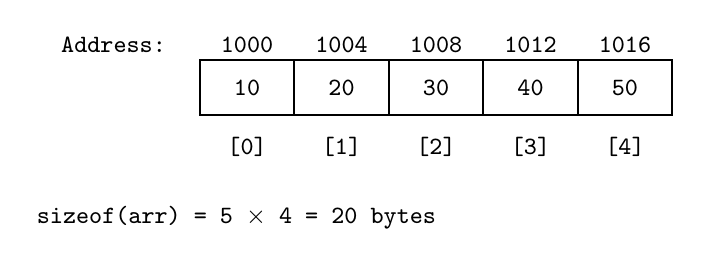
\begin{tikzpicture}[thick, font=\ttfamily\small]
			
			% Etichetta "Address:"
			\node[anchor=east] at (-0.3, 0.9) {Address:};
			
			% Indirizzi di memoria sopra le celle
			\node at (0.6, 0.9) {1000};
			\node at (1.8, 0.9) {1004};
			\node at (3.0, 0.9) {1008};
			\node at (4.2, 0.9) {1012};
			\node at (5.4, 0.9) {1016};
			
			% Celle dell'array (valori memorizzati)
			\draw[fill=white] (0, 0) rectangle (6, 0.7);
			\foreach \x in {1.2, 2.4, 3.6, 4.8} {
				\draw (\x, 0) -- (\x, 0.7);
			}
			\node at (0.6, 0.35) {10};
			\node at (1.8, 0.35) {20};
			\node at (3.0, 0.35) {30};
			\node at (4.2, 0.35) {40};
			\node at (5.4, 0.35) {50};
			
			% Indici sotto le celle
			\node at (0.6, -0.4) {[0]};
			\node at (1.8, -0.4) {[1]};
			\node at (3.0, -0.4) {[2]};
			\node at (4.2, -0.4) {[3]};
			\node at (5.4, -0.4) {[4]};
			
			% Formule e calcoli in basso
			\node[anchor=west] at (-2.2, -1.3) {sizeof(arr) = 5 $\times$ 4 = 20 bytes};
			
		\end{tikzpicture}
	\end{center}
	
	Giusto per accennarlo, si possono definire anche array bidimensionali, dove ogni elemento di un array bidimensionale è a sua volta un array. Un array bidimensionale viene spesso visto come una matrice di \texttt{n} righe ed \texttt{m} colonne
	\begin{center}
		\texttt{int matrice[2][3] = \{\{1,2,3\}, \{4,5,6\}\}}
	\end{center}
	E come si può immaginare, per accedere ad una cella della matrice, si deve indicizzare sia per riga che per colonna. Ad esempio per ottenere l'elemento \texttt{4} devo scrivere \texttt{matrice[1][0]}.
	
	\section{Le stringhe}
	Al contrario di altri linguaggi, come ad esempio il Python o Java, le stringhe non sono un tipo nativo in C.
	Queste sono definite come un array di caratteri, che ha come ultimo carattere il carattere di escape \texttt{'$\backslash$0'}, che indica il \textit{fine parola}.
	La definizione di una stringa avviene dunque come segue:
	\begin{center}
		\texttt{char saluto[] = "Ciao";}
	\end{center}
	E tale stringa sarà rappresentata in memoria esattamente come abbiamo visto rappresentare un'Array, con l'aggiunta del carattere '$\backslash$0' citato prima. In questo caso avremo dunque 
	\begin{center}
		\texttt{['C', 'i', 'a','o','$\backslash$0']}
	\end{center}
	
	\subsection{Funzioni per le stringhe}
	Il linguaggio C mette a disposizione una libreria \texttt{string.h} che dispone anche di alcune funzioni utili nel lavorare con le stringhe.
	
	\begin{itemize}
		\item \textbf{Controllare la lunghezza di una stringa}: si utilizza \texttt{strlen} al contrario del classico metodo \texttt{sizeof} utilizzato per tutti gli altri tipi di variabile. Questo in quanto \texttt{sizeof} conta anche il carattere di fine riga.
		
		\item Per \textbf{copiare una stringa} all'interno di un'altra possiamo usare la funzione \texttt{strcpy}, che però non effettua alcun controllo sulla lunghezza della stringa di destinazione e su eventuali overflow. Il metodo consigliato è dunque \texttt{strncpy}, considerato più sicuro in quanto implementa tali controlli.
		
		\item Per \textbf{confrontare due stringhe} si utilizza il metodo \texttt{strcmp}, che prende come parametri due stringhe e restituisce \texttt{0 se le stringhe sono uguali}, \texttt{1 altrimenti}.
	\end{itemize}
	
	\section{I puntatori}
	Uno dei punti di forza, se non \textit{il} punto di forza del linguaggio C è proprio la flessibilità riguardo al controllo sulla memoria.
	Gran parte di questa gestione è garantita anche grazie ai \textbf{puntatori}, ovvero delle \textbf{variabili il cui valore è un indirizzo di memoria}.
	La dicharazione è molto semplice: se abbiamo una variabile di tipo \texttt{int} e vogliamo dichiarare un puntatore a quella variabile intera, lo faremo semplicemente aggiungendo un asterisco accanto al nome del tipo, dunque \texttt{int*}. Vale ovviamente per ogni tipo di variabile. Chiaramente bisogna mantenere \textbf{coerenza} tra il tipo della variabile che vogliamo puntare e il tipo del puntatore.
	\smallbreak
	Strettamente legato al concetto di puntatore è il concetto di indirizzo. Per prendere l'indirizzo appartenente ad una variabile utilizziamo l'operatore \texttt{\&}.
	\begin{center}
		\texttt{int x = 42;}\\
		\texttt{int* p = \$x}
	\end{center}
	Inoltre, se utilizziamo di nuovo l'operatore \texttt{*} davanti ad un puntatore, faremo riferimento al \textbf{valore contenuto nell'indirizzo di memoria puntato da quel puntatore.}
	\begin{center}
		\texttt{int x = 42;}\\
		\texttt{int* p = \$x}\\
		\texttt{printf("\%d", *p)} // Out: 42
	\end{center}
	Volendo, possiamo inizializzare un puntatore al valore speciale \texttt{NULL}, per indicare che non punta a nulla.
	
	\begin{osservazione}{Puntatori \texttt{void*}}{}
		In alternativa a quanto visto prima, se vogliamo definire un puntatore che nel corso del programma può fare riferimento a tipi di variabili differenti (non è una good practice, però), potremmo definire un puntatore come \texttt{void*}.
		In questo modo il nostro puntatore potrà puntare all'indirizzo di memoria di qualsiasi variabile, tuttavia \textbf{non} potremmo usare l'operatore \texttt{*} per accedere al valore dell'indirizzo puntato da quel puntatore.
		Dovremo fare un casting esplicito al tipo della variabile puntata.
		\begin{center}
			\texttt{int x = 42;}\\
			\texttt{void* p = \&x}\\
			\texttt{printf("\%d", (int*)*p)}
		\end{center}
	\end{osservazione}
	
	Possiam anche definire dei puntatori \textbf{costanti}, ovverosia che possono cambiare il valore (cioè l'indirizzo) memorizzato al proprio interno, ma \textbf{non può cambiare il valore} associato a quell'indirizzo.
	
	\subsection{Aritmetica dei puntatori}
	Di seguito alcune nozioni importanti su come funzionano i puntatori con gli Array e il tipo di operazioni aritmetiche che possonoe essere svolte sui puntatori.
	\begin{itemize}
		\item Un puntatore p ad un Array A punterà \textbf{sempre} al primo elemento di quell'array (dunque \texttt{int* p = arr}) è come dire \texttt{int* p = \&arr[0]}.
		
		\item Quando incrementiamo un puntatore di un'unità, il valore dell'indirizzo aumenta della \texttt{sizeof} del tipo della variabile puntata. Ad esempio, se abbiamo un puntatore \texttt{double* p = \&x} e facciamo \texttt{p++}, il valore dell'indirizzo di memoria andrà avanti della \texttt{sizeof(double)}, ovvero il numero di byte richiesti in memoria per memorizzare un double.\\
		Questo può essere un modo alternativo per iterare lungo gli elementi di un Array.
		
		\item Sottraendo il valore di due puntatori \texttt{p1, p2} (gli indirizzi di memoria, dunque), otteniamo come risultato \textbf{il numero di elementi compresi tra p1 e p2}.\\ Attenzione! Non la dimensione complessiva di quegli elementi, ma proprio il numero di elementi in mezzo! Ad esempio:
		\begin{center}
			\texttt{int arr[5] = {1,2,3,4,5}}\\
			\texttt{int* secondo = \&arr[1]}\\
			\texttt{int* ultimo = \&arr[4]}\\
			\texttt{$\backslash\backslash$ ultimo - secondo = 2}
		\end{center}
		
		\item Possono essere effettuate operazioni di comparazioni tra puntatori, e funzionano come possiamo aspettarci.
	\end{itemize}
	
	\section{La gestione della memoria}
	Ogni programma scritto in C organizza la propria memoria nel modo descritto dal diagramma sottostante.
	\begin{center}
		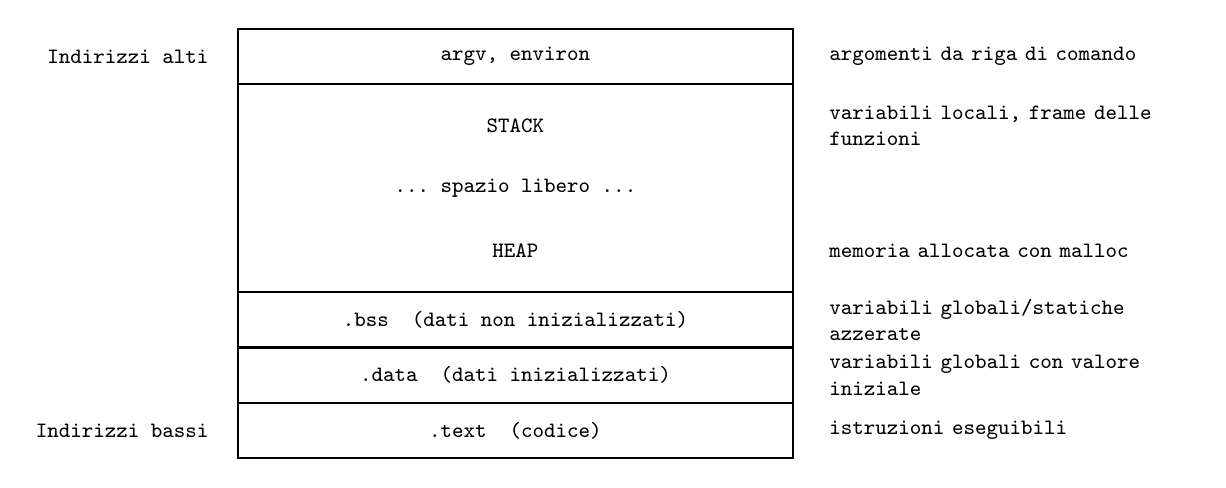
\begin{tikzpicture}[thick, font=\ttfamily\small, scale=0.88, transform shape]
			
			\def\boxW{8.0}
			
			% Box principale esterno
			\draw[fill=white] (0, 0) rectangle (\boxW, 6.2);
			
			% Separazioni orizzontali interne
			\draw (0, 0.8) -- (\boxW, 0.8);
			\draw (0, 1.6) -- (\boxW, 1.6);
			\draw (0, 2.4) -- (\boxW, 2.4);
			\draw (0, 5.4) -- (\boxW, 5.4);
			
			% --- TESTI INTERNI AL BOX (centrati orizzontalmente) ---
			\node at (\boxW/2, 5.8) {argv, environ};
			
			\node at (\boxW/2, 4.8) {STACK};
			\node at (\boxW/2, 3.9) {\dots\ spazio libero \dots};
			\node at (\boxW/2, 3.0) {HEAP};
			
			\node at (\boxW/2, 2.0) {.bss \ (dati non inizializzati)};
			\node at (\boxW/2, 1.2) {.data \ (dati inizializzati)};
			\node at (\boxW/2, 0.4) {.text \ (codice)};
			
			% --- INDIRIZZI A SINISTRA ---
			\node[anchor=east] at (-0.3, 5.8) {Indirizzi alti};
			\node[anchor=east] at (-0.3, 0.4) {Indirizzi bassi};
			
			% --- DESCRIZIONI A DESTRA (con text width per evitare uscite dal foglio) ---
			\tikzset{desc/.style={anchor=west, align=left, text width=5.2cm}}
			
			\node[desc] at (\boxW + 0.4, 5.8) {argomenti da riga di comando};
			\node[desc] at (\boxW + 0.4, 4.8) {variabili locali, frame delle funzioni};
			\node[desc] at (\boxW + 0.4, 3.0) {memoria allocata con malloc};
			\node[desc] at (\boxW + 0.4, 2.0) {variabili globali/statiche azzerate};
			\node[desc] at (\boxW + 0.4, 1.2) {variabili globali con valore iniziale};
			\node[desc] at (\boxW + 0.4, 0.4) {istruzioni eseguibili};
			
		\end{tikzpicture}
	\end{center}
	
	In questa sezione andremo a discutere, più o meno nel dettaglio, il funzionamento di queste componenti.
	
	\subsection{Lo Stack}
	Lo \textbf{Stack} è una regione di memoria utilizzato principalmente per la memorizzazione delle funzioni e delle variabili a loro associate (che siano essi parametri passati alle funzioni o variabili locali dichiarate al loro interno).
	Come suggerisce il nome, questa memoria opera in modalità \textbf{LIFO}, ovvero l'ultima funzione ad essere inserita sulla pila è anche la prima ad uscire (intuitivamente, se abbiamo una funzione A che chiama al suo interno una funzione B, la funzione B verrà terminata prima della sua chiamante, e dunque rimossa prima dalla pila).
	\smallbreak
	Ogni chiamata di funzione crea un cosiddetto \textbf{stack frame}, ovvero un blocco di celle di memoria in cui vengono memorizzati dei dati riguardanti la funzione:
	\begin{itemize}
		\item \textbf{Gli argomenti passati alla funzione} che, se sono pochi, vengono memorizzati all'interno di speciali registri, altrimenti vengono inseriti nello stack frame.
		
		\item L'indirizzo della prossima istruzione da eseguire \textbf{dopo} la fine dell'esecuzione della funzione. Questo valore viene memorizzato in quanto anche la funzione chiamata dovrà seguire un suo valore di Program Counter.
		
		\item Un puntatore, detto \textbf{frame pointer} che punta all'inizio dello \textbf{stack frame della funzione chiamante}.
		
		\item \textbf{Variabili locali} alla funzione.
	\end{itemize}
	
	Inoltre, nella gestione della memoria Stack, vengono utilizzati due registri:
	\begin{itemize}
		\item \textbf{Stack pointer}, che punta alla cima dello stack.
		
		\item \textbf{Frame pointer} che, come già detto, punta ad uno specifico stack frame.
	\end{itemize}
	
	Come si potrebbe intuire, un eccessivo numero di chiamate di funzione può portare al \textbf{riempimento eccessivo dello stack}. In quel caso si parla di \textbf{Stack Overflow}, e può accadere ad esempio quando si hanno troppe chiamate ricorsive ad una funzione.
	
	\begin{osservazione}{Il compilatore e lo Stack}{}
		Quando un programma viene compilato, il compilatore analizza ogni singola funzione, con i suoi parametri, variabili locali e tipi di ritorno e conosce già la dimensione dello stack frame associato a quella funzione.
	\end{osservazione}
	
	\subsection{Lo Heap}
	Lo \textbf{Heap} è una regione di memoria dedicata all'allocazione dinamica e \textbf{manuale} delle variabili da parte dell'utente. A differenza dello Stack, la dimensione dello Heap non è conosciuta a compilazione, ma rappresenta comunque un'area di memoria molto vasta.\\
	Le variabili in C possono essere manualmente allocate tramite appositi comandi, che permetteranno alle variabili di essere memorizzate nell'Heap e non in altre aree di memoria.\\
	I comandi predisposti sono i seguenti:
	\begin{description}
		\item [\texttt{malloc(n)}:] serve ad allocare manualmente un blocco di \texttt{n} bytes in memoria. Ad esempio, se volessimo allocare dinamicamente un array di 5 elementi potremmo scrivere \texttt{int* arr = malloc(5 * sizeof(int))}.
		
		\item[\texttt{calloc(n, size)}:] serve ad allocare \texttt{n} byte, ognuno di dimensione \texttt{size} e di inizializzare tutti quei byte al valore di default per quel tipo di dato. Tenendoci sull'esempio dell'Array di prima, se facessimo \texttt{int* arr = calloc(5, sizeof(int))} e provassimo a mandare a schermo l'Array otterremmo \texttt{[0, 0, 0, 0, 0]}.
		
		\item[\texttt{realloc(ptr, new\_size)}:] serve per riallocare un blocco di memoria precedentemente allocato. Supponendo di aver definito con \texttt{malloc} prima un array \texttt{arr} di 5 elementi interi, ma ci siamo resi conto che ci serve spazio per almeno 8 elementi, possiamo semplicemente fare \texttt{int* tmp = realloc(arr, 8 * sizeof(int))}.
		
		\item[\texttt{free(ptr)}:] fondamentale, serve a liberare un puntatore di memoria precedentemente allocato manualmente. Importantissimo è anche impostare il puntatore a \texttt{NULL} dopo averlo liberato.
	\end{description}
	
	Allocando e deallocando frequentemente nella memoria Heap si potrebbe verificare la cosiddetta \textbf{frammentazione della memoria}, ossia avere complessivamente molta memoria libera, ma a blocchi separati da memoria utilizzata.
	La seguente figura renderà bene il concetto:
	\begin{figure}[htbp]
		\centering
		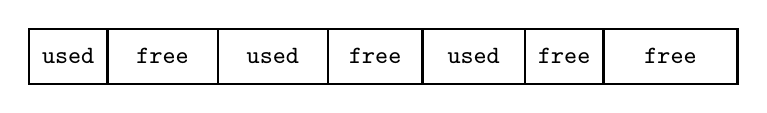
\begin{tikzpicture}[thick, font=\ttfamily\small]
			
			\def\totalW{9.0}
			
			% Contorno esterno
			\draw[fill=white] (0, 0) rectangle (\totalW, 0.7);
			
			% Divisioni interne e testi delle celle
			% used: 0 - 1.0
			\draw (1.0, 0) -- (1.0, 0.7);
			\node at (0.5, 0.35) {used};
			
			% free: 1.0 - 2.4
			\draw (2.4, 0) -- (2.4, 0.7);
			\node at (1.7, 0.35) {free};
			
			% used: 2.4 - 3.8
			\draw (3.8, 0) -- (3.8, 0.7);
			\node at (3.1, 0.35) {used};
			
			% free: 3.8 - 5.0
			\draw (5.0, 0) -- (5.0, 0.7);
			\node at (4.4, 0.35) {free};
			
			% used: 5.0 - 6.3
			\draw (6.3, 0) -- (6.3, 0.7);
			\node at (5.65, 0.35) {used};
			
			% free: 6.3 - 7.3
			\draw (7.3, 0) -- (7.3, 0.7);
			\node at (6.8, 0.35) {free};
			
			% free: 7.3 - 9.0 (ultimo blocco più largo)
			\node at (8.15, 0.35) {free};
			
		\end{tikzpicture}
		\caption{Frammentazione della memoria nell'Heap.}
		\label{fig:heap_fragmentation}
	\end{figure}
	
	\subsection{Errori di memoria}
	Spesso è proprio la libertà con la gestione della memoria conferitaci dal linguaggio ad essere causa della maggior parte degli errori che si incontrano nei programmi.
	Esempi degli errori più classici possono essere:
	\begin{description}
		\item[Perdita di memoria:] si verifica quando ci dimentichiamo di liberare una locazione di memoria ormai inutilizzata.
		
		\item[Doppia chiamata di \texttt{free()}:] si verifica quando chiamiamo \texttt{free()} due volte consecutive sullo stesso puntatore, senza averlo prima impostato a \texttt{NULL}.
		
		\item[Usare un puntatore dopo averlo liberato]
		
		\item [Puntatori fantasma:] si verifica quando ad un puntatore vengono restituiti valori di variabili locali a funzioni.
		
		\item[Puntatori non inizializzati:] quando si dichiara un puntatore e non lo si inizializza a nessun valore, questo punta ad un indirizzo inutilizzato dal programma ma che potrebbe comunque servire in futuro. E' sempre buona pratica inizializzare i puntatori almeno a \texttt{NULL}.
		
		\item[Scrittura oltre i limiti di un Array:] quando si prova ad accedere ad indici inesistenti di un Array (es: se \texttt{int arr[5]}, non esisterà l'elemento \texttt{arr[5]} in quanto il conteggio degli indici parte da 0).
		
		\item[Variabili inizializzate:] una variabile non inizializzata contiene un qualsiasi valore presente precedentemente nello stack.
		
	\end{description}
	
	Esistono degli strumenti di compilazione come \texttt{valgrind} o \texttt{AddressSanitizer}, ma li citiamo solo per nozione e non per approfondirli.
	
	\section{La traduzione da sorgente ad eseguibile}
	Il processo di traduzione di un programma C nel suo eseguibile è un'operazione molto lunga e articolata in diverse fasi. In questa sezione vedremo quali sono queste sezioni e le discuteremo una per una.
	Di seguito un'immagine rappresentante la classica struttura di compilazione di un programma in C:
	\begin{figure}[htbp]
		\centering
		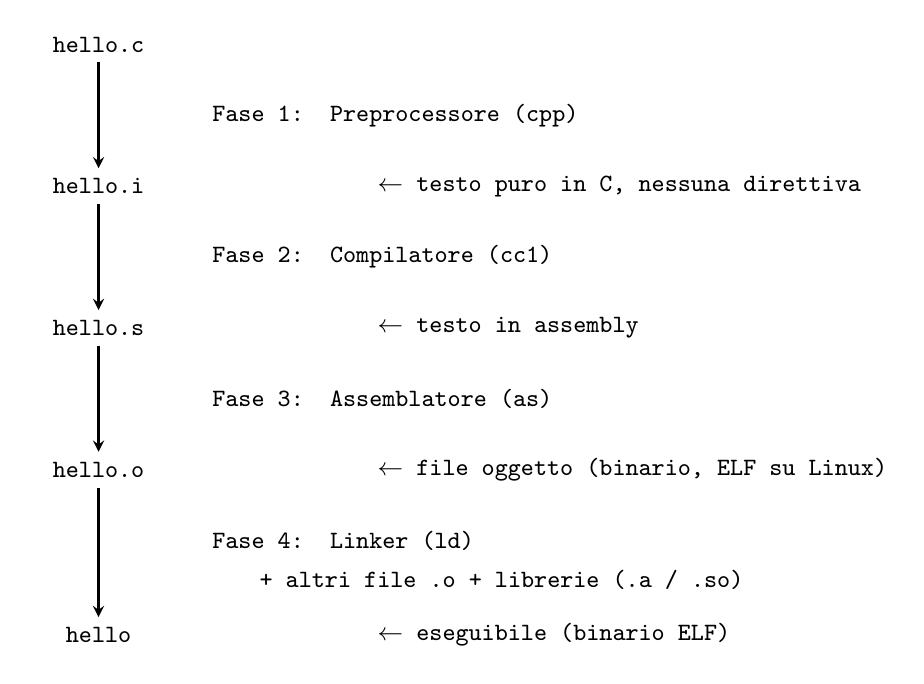
\begin{tikzpicture}[thick, font=\ttfamily\small, >=stealth]
			
			% Stile per le etichette dei file a sinistra
			\tikzset{
				filelabel/.style={
					anchor=east,
					minimum width=1.8cm,
					align=right
				},
				stage/.style={
					anchor=west,
					align=left
				},
				desc/.style={
					anchor=west,
					align=left
				}
			}
			
			% Posizionamento dei file (da hello.c fino all'eseguibile hello)
			\node[filelabel] (c) at (0, 0)    {hello.c};
			\node[filelabel] (i) at (0, -1.8) {hello.i};
			\node[filelabel] (s) at (0, -3.6) {hello.s};
			\node[filelabel] (o) at (0, -5.4) {hello.o};
			\node[filelabel] (e) at (0, -7.5) {hello};
			
			% Frecce verticali di transizione
			\draw[->] (c.south) -- (i.north);
			\draw[->] (i.south) -- (s.north);
			\draw[->] (s.south) -- (o.north);
			\draw[->] (o.south) -- (e.north);
			
			% Fase 1: Preprocessore
			\node[stage] at (0.4, -0.9) {Fase 1: Preprocessore (cpp)};
			\node[desc]  at (2.5, -1.8) {$\leftarrow$ testo puro in C, nessuna direttiva};
			
			% Fase 2: Compilatore
			\node[stage] at (0.4, -2.7) {Fase 2: Compilatore (cc1)};
			\node[desc]  at (2.5, -3.6) {$\leftarrow$ testo in assembly};
			
			% Fase 3: Assemblatore
			\node[stage] at (0.4, -4.5) {Fase 3: Assemblatore (as)};
			\node[desc]  at (2.5, -5.4) {$\leftarrow$ file oggetto (binario, ELF su Linux)};
			
			% Fase 4: Linker
			\node[stage] at (0.4, -6.3) {Fase 4: Linker (ld)};
			\node[stage] at (1.0, -6.8) {+ altri file .o + librerie (.a / .so)};
			\node[desc]  at (2.5, -7.5) {$\leftarrow$ eseguibile (binario ELF)};
			
		\end{tikzpicture}
		\caption{Pipeline di compilazione di un programma in C: dal sorgente (\texttt{.c}) all'eseguibile finale (\texttt{hello}) attraverso le quattro fasi fondamentali.}
		\label{fig:c_compilation_pipeline}
	\end{figure}
	
	\subsection{Il preprocessore}
	Si tratta del primissimo stadio dell'operazione di compilazione, e si occupa sostanzialmente di \textbf{manipolare il testo del programma} che abbiamo scritto. Parlando in modo più tecnico, si occupa di:
	\begin{itemize}
		\item Gestire tutti gli \texttt{\#include}. Questo viene fatto \textbf{copiando e incollando} il codice del file incluso all'interno del nostro file.
		
		\item Sostituire tutti i \texttt{\#define} con la corrispondente sostituzione scelta. Il comando \texttt{\#define MAX 100} \textit{alias} per una variabile all'interno del nostro programma. Nell'esempio fornito stiamo solo definendo un valore speciale \texttt{MAX} che vale 100, ma potremmo anche fare in modo che d'ora in poi nel nostro codice non dovremmo più dichiarare gli interi come \texttt{int} bensì come \texttt{intero} scrivendo semplicemente \texttt{\#define intero int}.
		
		\item Rimozione dei commenti sostituendoli con un singolo spazio bianco.
	\end{itemize}
	Questa fase trasforma il file \texttt{hello.c -> hello.i}.
	
	\subsection{La compilazione}
	Si tratta della fase che si occupa di \textbf{tradurre il codice scritto in C nelle corrispettive direttive scritte in Assembly}.
	Anche se un progetto include più file, ogni file con estensione .c viene compilato separatamente.
	Questa fase trasforma il file \texttt{hello.i -> hello.s/asm}
	
	\subsection{L'assemblaggio}
	Fase in cui entra in gioco il cosiddetto \textbf{assembler}, che si occupa di \textbf{convertire il testo scritto in Assembly in istruzioni macchina}. Non entreremo nel dettaglio di quale corrispondenza viene scelta a livello di bit, ma ciò dipende dal tipo di architettura della macchina (CISC/RISC come visto nella sezione~\ref{sec:instruction_set_architecture}). Questa fase genera il file \texttt{hello.s/asm -> hello.o}.
	
	\subsection{Il linking}
	Si tratta della fase finale del processo di traduzione, e si occupa sostanzialmente di \textbf{unire tutti i file oggetto del progetto in un singolo file eseguibile}.
	In particolare, vengono fatte queste operazioni intermedie:
	\begin{itemize}
		\item \textbf{Risoluzione dei simboli:} se ad esempio nel file \texttt{main.c} chiamiamo una funzione \texttt{calcola(a, b)}, il linker si occuperà di cercare in tutti i file oggetto una funzione con quel nome. In caso non dovesse trovarla, solleverà un errore tipo \texttt{undefined reference to 'calcola'}.
		
		\item \textbf{Riallocazione:} unisce tutti i file di codice in una singola sezione \texttt{.text} e tutte le sezioni dati in una sezione \texttt{.data}.
	\end{itemize}
	
	Alla fine di questo processo di traduzione viene finalmente \textbf{generato il file eseguibile}.
	
	\subsection{Librerie statiche e dinamiche}
	Durante l'operazione di linking, possono essere generati due tipi diversi di librerie.
	\begin{description}
		\item [Libreria statica:] si tratta di un file con estensione \texttt{.a} (che sta appunto per \textit{archivio}) che contiene una collezione di file oggetto. Durante il processo di linking, \textit{tutto} il codice di questa libreria viene copiato all'interno del programma principale.\\
		
		\item[Libreria dinamica:] si tratta di un file con estensione \texttt{.so} pensato per essere condiviso tra più file diversi. Si tratta di un'ottima scelta quando non si vuole far crescere la dimensione dell'eseguibile. Il grande vantaggio sta nel fatto che la copia delle funzioni utili non avviene a compilazione, bensì quando una funzione viene chiamata (il linker si occupa solo di inserire dei riferimenti per ogni funzione e il file in cui questa è definita).
	\end{description}
	
	\chapter{Processi e API di sistema}
	Abbiamo già definito il concetto di \textit{processo} nei capitoli precedenti, ma in questo capitolo ne vedremo meglio la natura, come creare processi, come eseguirli, ecc...
	
	\section{L'astrazione dei processi}
	Un processo è un'istanza di un programma in esecuzione, che comprende i seguenti parametri:
	\begin{itemize}
		\item Il \textbf{codice} che deve essere eseguito.
		
		\item Il valore corrente del \textbf{Program Counter}.
		
		\item I contenuti dei \textbf{registri della CPU}.
		
		\item Uno \textbf{spazio di memoria virtuale} a cui accedere (ovverosia il suo stack, il suo heap, ...)
		
		\item Gli identificativi ai file su cui il processo deve lavorare.
		
		\item Un \textbf{identificativo univoco di processo}, chiamato \textbf{ProcessID (PID)}.
	\end{itemize}
	
	In base alla filosofia secondo cui viene progettato il sistema operativo, questo può decidere di procedere secondo due strategie per allocare il processo in RAM:
	\begin{itemize}
		\item \textbf{Caricamento immediato}: appena il processo entra in esecuzione, tutti i suoi dati vengono caricati in memoria RAM. Si tratta di una soluzione facile ma poco efficiente, in quanto potrebbero venir caricate in memoria anche porzioni di codice mai utilizzate.
		
		\item \textbf{Caricamento pigro}: una sezione del processo viene caricata solo quando deve essere effettivamente utilizzata. Entreremo più nel tecnico di questa modalità quando parleremo di paging e memoria.
	\end{itemize}
	
	\section{Gli stati di un processo}
	Affinché lo scheduler del sistema operativo possa decidere quando mandare un processo in esecuzione, quando fermarlo e quando farne partire un altro, si attribuisce ad ogni processo uno \textbf{stato}.
	
	\begin{figure}[htbp]
		\centering
		\resizebox{0.70\linewidth}{!}{%
			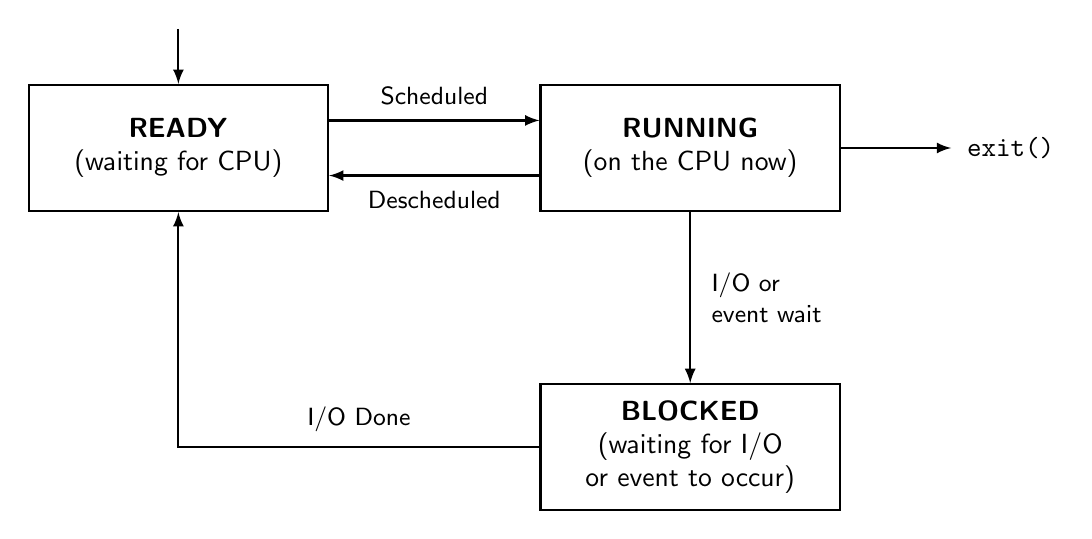
\begin{tikzpicture}[thick, >=latex]
				% Stile comune per gli stati del processo
				\tikzset{
					state/.style={
						draw,
						fill=white,
						minimum width=3.8cm,
						minimum height=1.6cm,
						align=center,
						font=\sffamily\normalsize
					}
				}
				
				% Stati principali
				\node[state] (ready) at (0, 3) {\textbf{READY}\\(waiting for CPU)};
				\node[state] (running) at (6.5, 3) {\textbf{RUNNING}\\(on the CPU now)};
				\node[state] (blocked) at (6.5, -0.8) {\textbf{BLOCKED}\\(waiting for I/O\\or event to occur)};
				
				% Freccia di ingresso verso READY
				\draw[->] (ready.north) ++(0, 0.7) -- (ready.north);
				
				% Transizioni tra READY e RUNNING
				\draw[->] ([yshift=0.35cm]ready.east) -- ([yshift=0.35cm]running.west)
				node[midway, above=2pt, font=\sffamily\small] {Scheduled};
				
				\draw[->] ([yshift=-0.35cm]running.west) -- ([yshift=-0.35cm]ready.east)
				node[midway, below=2pt, font=\sffamily\small] {Descheduled};
				
				% Transizione di uscita da RUNNING
				\draw[->] (running.east) -- ++(1.4, 0)
				node[right=2pt, font=\sffamily\normalsize] {\texttt{exit()}};
				
				% Transizione da RUNNING a BLOCKED
				\draw[->] (running.south) -- (blocked.north)
				node[midway, right=4pt, font=\sffamily\small, align=left] {I/O or\\event wait};
				
				% Transizione da BLOCKED a READY (percorso a L)
				\draw[->] (blocked.west) -| (ready.south)
				node[pos=0.25, above=2pt, font=\sffamily\small] {I/O Done};
			\end{tikzpicture}%
		}
		\caption{Diagramma a tre stati del ciclo di vita di un processo}
		\label{fig:stati_processo}
	\end{figure}
	
	Come si vede nella Figura \ref{fig:stati_processo} vi sono 3 possibili stati in cui un processo:
	\begin{description}
		\item [READY:] i processi in questo stato sono pronti per essere eseguiti, e attendono solo che lo scheduler li mandi in esecuzione. Dire che un proceso è "pronto" per essere eseguito vuol dire che \textbf{possiede tutte le risorse necessarie per eseguire la prossima istruzione}.
		
		\item[RUNNING:] è lo stato in cui si trova un \textbf{processo in esecuzione}. NOTA BENE: Ci può essere \textbf{solo un} processo in esecuzione alla volta su una singola CPU, in quanto è impossibile eseguire due processi simultaneamente.
		Se avessimo una CPU con $n$ core, si potrebbero eseguire simultaneamente $n$ processi, in quanto ogni core opererebbe come una CPU distinta con i suoi registri e i suoi stati.
		
		\item[BLOCKED:] i processi in questo stato sono quelli che \textbf{attendono una risorsa da un dispositivo di I/O}, senza la quale non potrebbero continuare l'esecuzione del programma (es: un input da tastiera). Viene definita una categoria a parte per quando si richiedono risorse esterne in quanto abbiamo visto come l'interfacciamento con dispositivi esterni sia un'operazione molto lenta (soprattutto rispetto ai cicli di clock della CPU). 
	\end{description}
	
	\begin{osservazione}{Transizione RUNNING $\rightarrow$ READY}{}
		Affinché un processo passi da READY a RUNNING è sufficiente che lo scheduler decida che "è arrivato il suo momento di eseguire".
		\smallbreak
		Ma per il contrario? Se l'esecuzione di un processo fila liscia, senza neanche richiesta di interfacciarsi con dispositivi esterni, entra il gioco quello che nei capitoli precedenti avevamo chiamato \textit{Timer Interrupt}, ovvero un timer di sistema che assegna ad ogni processo un certo intervallo di tempo per eseguire le sue istruzioni, dopodiché lo fa terminare per lasciare spazio ad altri processi.
	\end{osservazione}
	
	\section{Il Process Control Block (PCB)}
	Affinché il sistema operativo possa tenere traccia di tutti i dati relativi ad un processo, per ognuno di questi viene associata una particolare struttura dati chiamata \textbf{Process Control Block (PCB)}.\\
	Questa struttura contiene informazioni fondamentali riguardo al processo, come ad esempio:
	\begin{itemize}
		\item Il suo \textbf{PID}.
		
		\item Il suo \textbf{stato corrente}, secondo la logica vista poco fa.
		
		\item Il \textbf{puntatore alla pagina di memoria riservata al process} (\textbf{pagetable}).
		
		\item Lo \textbf{stato e il contenuto dei registri della CPU} (\textbf{trapframe}).\\
		Siccome abbiamo una sola CPU che può eseguire un processo alla volta, quando un processo passa dalla fase di esecuzione ad una qualsiasi altra fase, dovrà memorizzare i valori dei registri nel momento in cui l'esecuzione è stata interrotta, in modo che quando venga ripresa questa non riparta dall'inizio ma dall'ultimo "checkpoint".
	\end{itemize}
	
	Tutti i PCB dei processi inizializzati vengono memorizzati all'interno di una struttura dati chiamata \textbf{Process Table} che \textbf{risiede in memoria kernel} (in quanto deve essere lo scheduler del sistema operativo a decidere chi eseguire). Lo scheduler andrà poi a scansionare questa tabella in ricerca di processi con stato READY da mandare in esecuzione.
	
	\section{La gerarchia dei processi}
	Nei sistemi UNIX, i processi formano un albero in cui la radice è il processo \textbf{systemd} con PID = 1. Questo processo non può essere killato neanche volendo, in quanto è strettamente legato al funzionamento del kernel e del sistema operativo.\\
	La gerarchia dei processi è organizzata ad albero in quanto ogni processo può creare altri processi figli (con il comando \texttt{fork()}) e dunque ogni processo ha anche un padre (il cui valore si chiama \textbf{Parent ProcessID (PPID)}).
	
	\newpage
	\section{La funzione fork()}
	La funzione \texttt{fork()} è forse una delle funzioni più utili quando si va a lavorare con i processi, in quanto permette di \textbf{creare un nuovo processo}.\\
	Più precisamente, ci permette di \textbf{duplicare il PCB del processo padre}, ovvero il PCB del processo chiamante. Quest'operazione ci permetterà di allocare un PCB (dunque senza bisogno di conoscere la natura della struttura dati, astrazione!) e poi di modificarlo quasi a piacimento.
	\smallbreak
	Vediamo un esempio di utilizzo di \texttt{fork()} all'interno di un codice e commentiamolo:
	\begin{lstlisting}[language=C]
		int main() {
			int pid = fork();
			
			if (pid < 0) {
				perror("fork failed");
			} else if (pid == 0) {
				printf("Processo figlio con PID: %d", getpid());
			} else {
				printf("Processo padre con PID: %d", getpid());
			}
		}
	\end{lstlisting}
	Analizziamo ogni singola istruzione di questo codice che, seppur breve, ci dovrebbe aiutare a capire il funzionamento di \texttt{fork()}.
	\begin{enumerate}
		\item \textbf{Chiamata alla funzione fork()}: come abbiamo già detto, avendo mandato il programma in esecuzione, quello sarà un processo, supponiamo con PID = 1234. Chiamando \texttt{fork()} all'interno di questo processo, stiamo dicendo al sistema di creare un nuovo processo (dunque un nuovo PCB) che sia sostanzialmente una \textbf{copia} del PCB del processo chiamante (che sarà il padre di questo nuovo processo).
		
		\item \textbf{Cosa viene copiato nel PCB}: il PCB padre e PCB figlio avranno in comune l'area di memoria in cui è presente il codice binario da eseguire, ossia entrambi punteranno \textbf{allo stesso indirizzo di memoria}.\\
		Oltre a questo, non hanno altro in comune: avranno sì gli stessi valori delle variabili, ma solo perché i valori dei registri saranno stati copiati e incollati anche nel PCB figlio. Il processo figlio avrà le proprie aree di memoria stack e heap, dunque se provassero a modificare la stessa variabile non riuscirebbero ad agire sullo stesso valore in quanto sarebbero logicamente indipendenti. E' molto importante sapere che al processo figlio, ovviamente, viene assegnato un nuovo PID. Supponiamo 1235 per il nostro esempio.
		
		\item A questo punto, avviene una sezione critica: avendo copiato nel processo figlio lo stato di \textbf{tutti} i registri, sarà stato copiato anche il valore del Program Counter, e dunque processo padre e figlio riprenderanno \textbf{dallo stesso identico punto}.
		
		\item Discutiamo ora il valore di ritorno della funzione \texttt{fork()}: prima di restituire un valore, viene eseguita la funzione e dunque creato il processo figlio. A questo punto, come abbiamo detto, i due processi condivideranno la stessa area di memoria per il codice ma non la stessa per le variabili. Qui il sistema fa una cosa interessante:
		\begin{itemize}
			\item All'interno del processo figlio, il valore di ritorno della funzione sarà \textbf{categoricamente 0}. Si tratta di una convenzione stabilita per indicare che il processo corrente è figlio di uno già esistente.
			\item All'interno del processo padre, la funzione \texttt{fork()} restituirà il PID del processo appena creato.
		\end{itemize}
		Ma come è possibile che una singola funzione restituisca un valore diverso a due processi diversi?\\
		Questo avviene in quanto, dopo aver creato le aree di memoria dedicate al processo figlio, il valore di ritorno della funzione verrà messo per ogni processo all'interno di uno speciale registro della CPU. Avendo due registri diversi, uno per il padre e uno per il figlio, è possibile creare questa "voluta discrepanza" tra i valori di ritorno.
		
		\item Una volta che la chiamata a \texttt{fork()} (supponiamo) è andata a buon fine, quindi, i possibili valori assumibili dalla nostra variabile intera sono \textbf{0 per il processo figlio} e $\mathbf{>0}$ \textbf{per il processo padre.}\\
		Questa è la ragione per cui inseriamo quei controlli all'interno del codice: \textbf{non avendo garanzia di chi partirà per primo con l'esecuzione}, e magari volendo separare tra le operazioni che può compiere il figlio e quelle del padre, l'unico modo è necessariamente controllare il valore restituito da \texttt{fork()}.
	\end{enumerate}
	
	Come ci si può aspettare, la funzione di libreria C \texttt{fork()} nasconde sottobanco una chiamata di sistema alla funzione \texttt{sys\_fork()}. Viene effettuata una chiamata di sistema in quanto abbiamo già detto che la Process Table in cui sono memorizati i PCB dei vari processi risiede in memoria kernel, e dunque è strettamente vietato far accedere quell'area di memoria da parte di un'istruzione utente.
	\smallbreak
	Inoltre, come è stato già detto nella descrizione del flusso di esecuzione del processo \texttt{fork()}, è impossibile predirre chi, tra il padre o il figlio, verrà eseguito prima come processo. Tutto dipende dallo scheduler e dalla priorità attribuita ad ogni processo. E' dunque sconsigliato scrivere porzioni di codice \textit{assumendo che un processo venga eseguito prima dell'altro}.
	
	Un modo per forzare l'esecuzione del processo figlio prima del processo padre è quello di mettere "a dormire" il processo padre, usando la funzione di libreria \texttt{sleep()}.
	\begin{lstlisting}[language=C]
		int main() {
			int pid = fork();
			
			if (pid < 0) {
				perror("errore nella fork");
			} else if (pid == 0) {
				// ESEGUO OPERAZIONI FIGLIO
			} else  {
				sleep(1);
				// ESEGUO OPERAZIONI PADRE
			}
		}
	\end{lstlisting}
	In questo modo stiamo forzatamente interrompendo per 1 secondo l'esecuzione del processo padre, tempo che per la CPU è enorme dato che esegue gli switch tra un processo e l'altro nell'ordine di nanosecondi. Questo modo è chiaramente molto grossolano, ed è una \textbf{bad practice} in quanto mette a dormire il padre anche se il processo figlio è stato eseguito per primo.
	\smallbreak
	
	Prima di concludere il discorso sul comando \texttt{fork()}, vediamo come si comportano multiple chiamate della funzione all'interno di un programma.\\
	Supponiamo di avere questo codice:
	\begin{lstlisting}[language=C]
		fork(); (1)
		fork(); (2)
		fork(); (3)
		printf("Hello, World!");
	\end{lstlisting}
	Ragioniamo: ad ogni chiamata di fork, il numero di processi viene duplicato, in quanto un padre crea un processo figlio.\\
	Alla chiamata (1), diventano 2 processi. Siccome l'esecuzione del codice per tutti i processi riparte dallo stesso punto grazie al valore del Program Counter, ciascuno dei due processi eseguirà anche la \texttt{fork()} del punto (2). Dato che avremo 2 processi ad eseguire una \texttt{fork()} e ognuno di questi genera 2 processi figli, alla fine di (2) avremo un totale di 4 processi. Come si può immaginare, ognuno dei 4 processi eseguirà un \texttt{fork()} duplicando il numero di processi, arrivando così ad 8 processi.	Vediamo dunque come il numero di processi finali è dato da $2^n$ dove $n$ è il numero di \texttt{fork()} eseguite.
	
	Dunque se volessimo mandare in crash il sistema operativo, ora sapremmo come fare:
	\begin{lstlisting}[language=C, caption={Codice per implementare la cosiddetta "fork bomb".}]
		while (1) {
			fork();
		}
	\end{lstlisting}
	Questo ciclo continua a creare processi finché non viene raggiunto il limite di processi memorizzabili all'interno della Process Table, e dunque il sistema operativo va in crash.\\
	Una possibile soluzione a questo problema sarebbe definire un limite massimo di processi generabili da un singolo utente.
	
	\subsection{La filosofia Copy-on-Write}
	In modo molto ingenuo, il comando \texttt{fork()} copierebbe l'intero spazio di memoria di un processo (che potenzialmente potrebbero essere anche diversi GB di memoria) in una nuova area riservata al processo figlio.\\
	I sistemi operativi moderni evitano questa pratica (proprio per evitare sprechi di memoria) implementando la cosiddetta filosofia \textbf{Copy-on-Write}:
	\begin{itemize}
		\item Alla creazione del nuovo processo, l'area di memoria a lui attribuita non è una copia di quella del processo padre, bensì gli viene attribuito lo \textbf{stesso indirizzo di memoria} della memory page del padre. Possiamo quindi dire che fino ad un certo momento condivideranno letteralmente la stessa risorsa, dato che viene passato l'indirizzo di questa.
		
		\item Quando uno dei due processi prova a modificare la suddetta area condivisa, viene sollevata una \textbf{Page Fault} dalla Memory Management Unit. Solo a questo punto viene creata la copia in memoria della pagina, che includerà le modifiche apportare dal processo che le ha richieste.\\
		A questo punto avremmo dunque due pagine di memoria separate:
		\begin{itemize}
			\item La pagina di memoria "originale", alla quale punta il processo che \textbf{non} ha provato a modificarla.
			
			\item La pagina di memoria \textit{copiata e modificata} dal processo che \textbf{ha} provato a modificarla.
		\end{itemize}
	\end{itemize}
	
	\section{La sincronizzazione dei processi con wait()}
	Come abbiamo detto e come si vuole ripetere, è impossibile determinare chi, tra il processo padre e quello figlio, riprenda l'esecuzione in seguito ad una \texttt{fork()}.\\
	Supponendo che il processo figlio termini prima di quello del padre, la memoria dedicata al processo figlio \textbf{non verrà eliminata}, bensì verrà mantenuta fino alla fine del processo padre. Il processo figlio verrà poi messo in uno stato detto \textbf{ZOMBIE}.\\
	Per fare in modo che questo problema non si presenti, il sistema operaivo mette a disposizione la funzione \texttt{wait()} che ci permette di fermare l'esecuzione del processo padre in attesa che i processi figli siano terminati.
	\smallbreak
	
	Vediamo di seguito la firma del metodo \texttt{wait()}, commentiamola, e poi vediamo un esempio di utilizzo nel codice.
	\begin{center}
		\texttt{int wait(int *wstatus);}
	\end{center}
	\begin{itemize}
		\item La funzione restituisce un valore intero che, se l'esecuzione di \texttt{wait()} è andata a buon fine, rappresenta il PID del processo figlio che è terminato.
		
		\item Il parametro \texttt{int *wstatus} è un modo intelligente per far restituire alla funzione un altro valore.\\
		Siccome non siamo su Python e non possiamo restituire tuple di valori, il segreto sta nel passare il puntatore ad una variabile non inizializzata e poi ci penserà la funzione \texttt{wait()} al suo interno a modificarla, memorizzandoci lo stato con cui si è conclusa l'esecuzione del processo figlio.
	\end{itemize}
	
	Vediamo ora un esempio concreto in un pezzo di codice.
	\begin{lstlisting}[language=C]
		int main() {
			int pid = fork();
			if (pid == 0) {
				printf("Sta eseguendo il figlio...");
				exit(42); // Un generico codice di uscita
			}
			
			// Adesso siamo nel parent e dobbiamo attendere che finisca il child
			int stato;
			int finito = wait(&stato);
			
			if (child_pid == -1) {
				perror("wait");
			} else {
				printf("Arrivo qui solo dopo che ho finito.")
			}
		}
	\end{lstlisting}
	Come vediamo, il valore assunto dalla variabile \texttt{finito} rappresenta il valore del processo figlio terminato. Nell'ottica di voler far eseguire prima il figlio del padre, questo è l'approccio che si deve attuare.\\
	Esiste anche la funzione \texttt{waitpid(int child\_pid)} che consente al processo padre di attendere la terminazione dell'esecuzione \textbf{solo del processo figlio che ha PID uguale a quello passato come parametro della funzione}.
	
	\section{La funzione exec()}
	La funzione \texttt{exec()} è una procedura fondamentale in quanto ci permette di sostituire il codice eseguito da un processo con un altro file binario contenente altro codice.\\
	Si tratta di una funzionalità molto utile, in quanto non risulta avere particolarmente senso far eseguire sia un processo che i suoi figli lo stesso file binario.
	\begin{osservazione}{Successo di exec()}{}
		Se la funzione \texttt{exec()} viene portata a termine con successo, il processo figlio non tornerà mai ad eseguire il processo padre in quanto avrà cambiato totalmente file binario.
	\end{osservazione}
	
	Una variante di \texttt{exec()} è la funzione \texttt{execvp(const char* file, char* const argv[])}, che prende come input il file binario di cui eseguire il codice ed eventuali argomenti che servono a tale programma per completare la sua esecuzione.\\
	Prendiamo ad esempio il seguente codice:
	\begin{lstlisting}[language=C, caption={Il comando ls serve a listare il contenuto della directory "$\backslash$tmp", e i vari argomenti che iniziano con '-' sono dei flag che compiono operazioni aggiuntive.}]
		char* args[] = {"ls", "-l" "-a", "\tmp", NULL};
		execvp("ls", args);
	\end{lstlisting}
	Il processo corrente inizierà ad eseguire il comando \texttt{ls}	(preso in questo caso dalle variabili di ambiente, ma solo perché è uno dei comandi di default di Linux) con i vari argomenti dell'array \texttt{args}. Il valore di terminazione per smettere di leggere argomenti è il valore speciale \texttt{NULL} all'interno dell'Array degli argomenti.
	\smallbreak
	
	Avendo visto il funzionamento sia per \texttt{fork()} che \texttt{exec()}, vediamo un esempio di programma che li combina.
	\begin{lstlisting}[language=C, caption={Esempio di uso combinato di fork() e execvp(). Si ignorano possibili errori per brevità.}]
		int main() {
			int pid = fork();
			if (pid == 0) {
				execvp("ls", {"\tmp", NULL})
			} else {
				printf("Processo padre.")
			}
		}
	\end{lstlisting}
	
	Avendo visto e compreso il funzionamento di questi due comandi, possiamo avere anche una visione più chiara di come funzioni un'istanza di terminale (shell), in quanto si basa su un loop di istruzioni molto preciso:
	\begin{enumerate}
		\item Far scrivere all'utente un comando. 
		
		\item Leggere il comando e dividerlo in token.
		
		\item Creare un processo figlio che si occupi di eseguire il comando (\texttt{fork()}).
		
		\item Far eseguire il comando al processo figlio (\texttt{execvp()}).
		
		\item Attendere che il processo figlio termini l'esecuzione del comando (\texttt{wait()}).
		
		\item Restituire il controllo al processo padre e ritornare all'inizio del loop.
	\end{enumerate}
	\begin{osservazione}{Reale funzionamento di una shell}{}
		Una vera shell in realtà consente anche all'utente di eseguire nuovi comandi mentre altri stanno continuando in background. Questo può avvenire inserendo il carattere \texttt{\&} alla fine di un comando, il che indicherà al sistema operativo di restituire il controllo all'utente subito dopo aver mandato in esecuzione il comando precedente.
	\end{osservazione}
	
	\section{Altre API di sistema}
	Di seguito un veloce elenco di altre API di sistema importanti ma non fondamentali come quelle descritte precedentemente.
	
	\begin{description}
		\item [exit():] si occupa di terminare un processo. E' presente in due varianti:
		\begin{itemize}
			\item \texttt{exit()}, che termina il processo in modo "lento" ma pulendo tutti i buffer e pulendo tutti gli stream.
			
			\item \texttt{\_exit()}, che termina il processo in modo veloce ma senza pulire buffer e stream.
		\end{itemize}
		
		\item[kill():] per inviare un segnale al processo figlio e "ucciderlo".
		
		\item[nice():] per aggiornare il livello di priorità di un processo. Tale livello è un numero intero che va da \textbf{-20} (\textbf{priorità massima}, solo il kernel) a \textbf{+19} (\textbf{priorità minima}, programmi utente).
		
		\item[pipe():] crea un canale di comunicazione tra due o più processi per permettere di condividere l'output di un processo con l'input di un altro. 
	\end{description}
	
	\chapter{Scheduling della CPU}
	Nei capitoli precedenti abbiamo accennato a come i sistemi moderni creino l'illusione di eseguire simultaneamente più processi "semplicemente" effettuando dei rapidissimi scambi di stato tra i processi in esecuzione.\\
	In questo capitolo vedremo più nel dettaglio il ruolo dello \textbf{scheduler}, ovverosia quel modulo del kernel che si occupa di decidere, mediante un accorto \textbf{algoritmo di scheduling}, l'ordine dei processi da mandare in esecuzione.
	\smallbreak
	
	L'obiettivo non sarà tuttavia fornire direttamente la soluzione adottata oggi dai sistemi moderni, bensì di guidare l'apprendimento imponendo dei vincoli e man mano rimuovendoli, per trovare standard sempre più efficaci.
	
	\section{Assunzioni sul carico di lavoro e metriche}
	Affinché lo scheduler possa organizzare i processi, bisogna definire il carico di lavoro e delle metriche secondo le quale stabilire questi confronti.
	
	\begin{definizione}{Carico di lavoro}{workload}
		Il carico di lavoro descrive:
		\begin{itemize}
			\item Quanti processi stanno attualmente venendo eseguiti dal sistema.
			
			\item L'istante di tempo in cui viene creato un nuovo PCB.
			
			\item \textbf{Quanto tempo} è richiesto per ogni processo.
			
			\item \textbf{Quando} il processo dovrà fare operazioni di I/O.
		\end{itemize}
	\end{definizione}
	
	\begin{osservazione}{Natura asincrona dei processi}{}
		E' doveroso fare un appunto sulla definizione soprastante.\\
		Per lo scheduler è \textbf{impossibile} predirre gli ultimi due punti, in quanto i processi sono di per sè un'unità asincrona in cui alcune cose non sono deterimistiche.
	\end{osservazione}
	
	\newpage
	Al fine di costruire il nostro percorso in maniera graduale verso un algoritmo di scheduling efficiente che funzioni per ogni sistema, dobbiamo partire letteralmente \textit{dalle basi}, facendo delle assunzioni \textbf{molto comode} sulla natura del workload:
	\begin{enumerate}
		\item Ogni processo richiede la \textbf{stessa quantità di tempo} per essere eseguito.
		
		\item Tutti i processi \textbf{arrivano allo stesso momento} ($t = 0$).
		
		\item Prima di cambiare processo deve essere \textbf{completamente terminato il corrente} (nessuna interruzione del processo).
		
		\item \textbf{Nessun} processo ha necessità di eseguire operazioni di \textbf{I/O}.
		
		\item Il \textbf{tempo di esecuzione} di ogni processo è \textbf{noto a priori}.
	\end{enumerate}
	Come vediamo sono delle assunzioni molto comode, che però piano piano andremo a calare per migliorare progressivamente l'algoritmo di scheduling che vogliamo progettare.
	\smallbreak
	
	Oltre a queste assunzioni, che si permetteranno di definire l'algoritmo, dobbiamo anche avere dei criteri per permetterci di stabilire se un algoritmo performa meglio di un altro.\\
	Abbiamo principalmente due metriche:
	\begin{description}
		\item [Tempo di completamento (Turnaround Time):] indica il tempo totale trascorso da quando il processo arriva al sistema a quando viene finito di eseguire.\\
		La formula per il calcolo di questo parametro è la seguente:
		\[
			T_\text{turnaround} = T_\text{fine\_processo} - T_\text{arrivo}
		\]
		Prendendo la media del tempo di completamento di tutti i processi schedulati, otteniamo l'importantissimo parametro di \textbf{Tempo di completamento medio}.
		
		\item[Tempo di risposta (Response Time):] rappresenta il tempo da quando un processo arriva al sistema a quando arriva ad essere eseguito per la prima volta. Sostanzialmente indica quanto tempo un processo rimane in coda prima di essere considerato.\\
		La formula per questo parametro è la seguente:
		\[
			T_\text{response} = T_\text{prima\_esecuzione} - T_\text{arrivo}
		\]
	\end{description}
	
	Questi appena descritti sono i parametri fondamentali nel calcolo dell'\textbf{equità} e delle \textbf{performance} di un algoritmo di scheduling.\\
	In particolare:
	\begin{description}
		\item [Equità (Fairness):] rappresenta in che misura il \textbf{tempo della CPU viene distribuito tra tutti i processi}. Un algoritmo è "\textbf{fair}" se garantisce a ogni processo di fare progressi regolari, evitando che qualche task rimanga bloccato ad aspettare per un tempo indefinito (starvation).
		
		\item[Prestazioni (Performance):] rappresenta la \textbf{capacità di minimizzazione del turnaround time o del response time}.
	\end{description}
	Si può facilmente intuire come queste due filosofie siano contrapposte, pertanto si deve scegliere cosa si deve prediligere maggiormente in un algoritmo, oppure trovare l'equilibrio più vantaggioso tra le due.
	
	\section{I primi passi: FIFO e SJF}
	Avendo messo le basi per la nostra analisi degli algoritmi di scheduling, partiamo dalle basi, con due delle strategie più semplici.
	
	\subsection{FIFO - First In, First Out}
	E' forse la schedule più semplice a cui si potrebbe pensare: \textbf{i primi processi ad entrare sono anche i primi a venir eseguiti}.\\
	Anche la sua implementazione risulta particolarmente semplice, in quanto consiste semplicemente nella gestione di una struttura dati \textit{coda}. Vediamo un semplice esempio di questo algoritmo usando anche le nostre 5 assunzioni precedenti.
	\smallbreak

	Supponiamo di avere tre job: \textbf{A}, \textbf{B} e \textbf{C} e che:
	\begin{itemize}
		\item Tutti arrivino allo stesso istante di tempo $t=0$.
		
		\item Tutti abbiano la stessa durata di $10s$.
	\end{itemize}
	
	\begin{figure}[htbp]
		\centering
		\resizebox{0.50\linewidth}{!}{%
			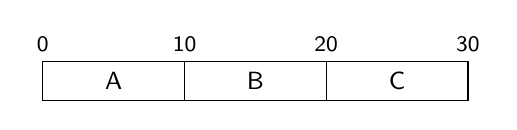
\begin{tikzpicture}
				% Tacche temporali
				\node[font=\sffamily\footnotesize] at (0, 0.22) {0};
				\node[font=\sffamily\footnotesize] at (1.8, 0.22) {10};
				\node[font=\sffamily\footnotesize] at (3.6, 0.22) {20};
				\node[font=\sffamily\footnotesize] at (5.4, 0.22) {30};
				
				% Blocchi dei Job (sottili, compatti e senza testo in grassetto)
				\draw[fill=white] (0, -0.5) rectangle (1.8, 0) node[midway, font=\sffamily\small] {A};
				\draw[fill=white] (1.8, -0.5) rectangle (3.6, 0) node[midway, font=\sffamily\small] {B};
				\draw[fill=white] (3.6, -0.5) rectangle (5.4, 0) node[midway, font=\sffamily\small] {C};
			\end{tikzpicture}%
		}
		\label{fig:linea_temporale_job}
	\end{figure}
	
	Andiamo adesso a calcolare il tempo di completamento per ogni processo e di conseguenza il tempo medio:
	\begin{itemize}
		\item A termina a $t=10$. Tempo di completamento = $10-0=10s$
		\item B termina a $t=20$. Tempo di completamento = $20-0=20s$
		\item C termina a $t=30$. Tempo di completamento = $30-0=30s$
	\end{itemize}
	Tempo di completamento medio: $\frac{10+20+30}{3} = 20s$.\\
	Non è un brutto tempo, solo che stiamo lavorando con delle ipotesi molto comode.
	\smallbreak
	
	Adesso, andiamo a rilassare l'Assunzione 1, quella sull'equa durata di tutti i processi.\\
	Proviamo a ridisegnare lo schema precedente supponendo ora che $A = 100s, B=C=10s$.
	
	\begin{figure}[htbp]
		\centering
		\resizebox{0.65\linewidth}{!}{%
			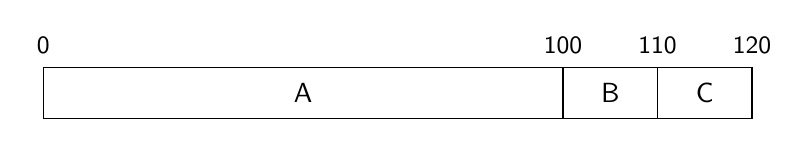
\begin{tikzpicture}
				% Tacche temporali ben spaziate e leggibili
				\node[font=\sffamily\small] at (0, 0.28) {0};
				\node[font=\sffamily\small] at (6.6, 0.28) {100};
				\node[font=\sffamily\small] at (7.8, 0.28) {110};
				\node[font=\sffamily\small] at (9.0, 0.28) {120};
				
				% Blocchi dei Job con altezza e larghezza calibrate per non schiacciare le etichette B e C
				\draw[fill=white] (0, -0.65) rectangle (6.6, 0) node[midway, font=\sffamily\normalsize] {A};
				\draw[fill=white] (6.6, -0.65) rectangle (7.8, 0) node[midway, font=\sffamily\normalsize] {B};
				\draw[fill=white] (7.8, -0.65) rectangle (9.0, 0) node[midway, font=\sffamily\normalsize] {C};
			\end{tikzpicture}%
		}
	\end{figure}
	Se andassimo ora a calcolare il tempo di esecuzione minimo per ogni processo, il risultato sarebbe ben diverso:
	\begin{itemize}
		\item A termina a $t=100$. Tempo di completamento = $100-0=100s$
		\item B termina a $t=110$. Tempo di completamento = $110-0=110s$
		\item C termina a $t=120$. Tempo di completamento = $120-0=120s$
	\end{itemize}
	Tempo di completamento medio: $\frac{100+110+120}{3} = 110s$.\\
	Vediamo che la situazione è cambiata, e questo dato che i processi corti $B$ e $C$ sono bloccati dietro il processo lungo $A$ e devono attenderne la fine. Nello studio degli algoritmi di scheduling, questo è detto \textbf{effetto convoglio}.
	
	\subsection{SJF - Shortest Job First}
	Per aggiustare questo effetto convoglio, evitando dunque che i procssi corti siano messi dopo uno più lungo di loro e rimangano bloccati, si attua la tecnica Shortest Job First (SJF) che, come suggerisce il nome, prevede di \textbf{eseguire per primo il processo più corto di tutti}.\\
	Tenendo conto di questa nuova strategia, se andiamo a ridisegnare il diagramma precedente con $A=100, B=C=10$, vediamo come le cose cambino anche solo eseguendo per primi i processi corti.
	\begin{figure}[htbp]
		\centering
		\resizebox{0.65\linewidth}{!}{%
			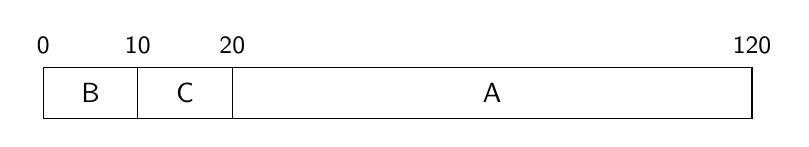
\begin{tikzpicture}
				% Tacche temporali ben spaziate e leggibili
				\node[font=\sffamily\small] at (0, 0.28) {0};
				\node[font=\sffamily\small] at (1.2, 0.28) {10};
				\node[font=\sffamily\small] at (2.4, 0.28) {20};
				\node[font=\sffamily\small] at (9.0, 0.28) {120};
				
				% Blocchi dei Job (SJF: B e C precedono A)
				\draw[fill=white] (0, -0.65) rectangle (1.2, 0) node[midway, font=\sffamily\normalsize] {B};
				\draw[fill=white] (1.2, -0.65) rectangle (2.4, 0) node[midway, font=\sffamily\normalsize] {C};
				\draw[fill=white] (2.4, -0.65) rectangle (9.0, 0) node[midway, font=\sffamily\normalsize] {A};
			\end{tikzpicture}%
		}
	\end{figure}
	\begin{itemize}
		\item B termina a $t=10$. Tempo di completamento = $10-0=10s$
		\item C termina a $t=20$. Tempo di completamento = $20-0=20s$
		\item A termina a $t=120$. Tempo di completamento = $120-0=120s$
	\end{itemize}
	Facendo la media, otteniamo $\frac{10+20+120}{3} = 50s$ il che è un tempo inferiore per più della metà rispetto a prima!\\
	\begin{osservazione}{Utilità del SJF}{}
		L'algoritmo SJF è \textbf{ottimale} per \textbf{minimizzare il tempo di completamento medio per processi che arrivano tutti allo stesso momento}.
	\end{osservazione}
	\smallbreak
	
	Avendo lavorato sulla prima assunzione, riguardante la durata dei processi e avendo trovato un algoritmo che ci permette di rendere efficiente lo scheduling con quell'ipotesi rilassata, andiamo a rilassare anche a rimuovere la seconda assunzione, riguardante il fatto che \textbf{tutti i processi arrivano allo stesso tempo}.\\
	Modifichiamo leggermente le variabili del nostro diagramma: $A=100, t=0; B=C=10, t=10$.
	
	\begin{figure}[htbp]
		\centering
		\resizebox{0.65\linewidth}{!}{%
			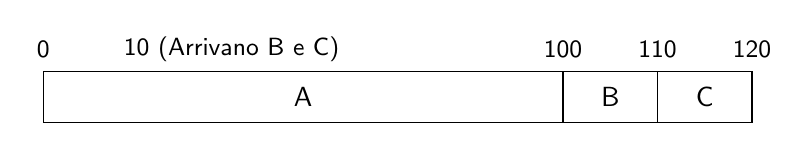
\begin{tikzpicture}
				% Tacche temporali e arrivo dei job
				\node[font=\sffamily\small] at (0, 0.28) {0};
				\node[font=\sffamily\small, anchor=west] at (0.9, 0.28) {10 (Arrivano B e C)};
				\node[font=\sffamily\small] at (6.6, 0.28) {100};
				\node[font=\sffamily\small] at (7.8, 0.28) {110};
				\node[font=\sffamily\small] at (9.0, 0.28) {120};
				
				% Blocchi di esecuzione dei Job
				\draw[fill=white] (0, -0.65) rectangle (6.6, 0) node[midway, font=\sffamily\normalsize] {A};
				\draw[fill=white] (6.6, -0.65) rectangle (7.8, 0) node[midway, font=\sffamily\normalsize] {B};
				\draw[fill=white] (7.8, -0.65) rectangle (9.0, 0) node[midway, font=\sffamily\normalsize] {C};
			\end{tikzpicture}%
		}
	\end{figure}
	Analizzando ciò che accade:
	\begin{enumerate}
		\item Al tempo $t=0$, l'unico processo presente è $A$ e dunque lo scheduler deve necessariamente scegliere quello.
		
		\item Al tempo $t=10$ arrivano B e C, ma siccome il SJF non offre nessun meccanismo per gestire l'interruzione di un processo, questi dovranno attendere che $A$ sia terminato prima di venir eseguiti.
	\end{enumerate}
	Vediamo dunque che in questa casistica, avendo semplicemente rilassato la seconda ipotesi, \textbf{l'effetto convoglio è tornato}.
	\begin{itemize}
		\item A termina a $t=100$. Tempo di completamento = $100-0=100s$
		\item B termina a $t=110$. Tempo di completamento = $110-10=100s$
		\item C termina a $t=120$. Tempo di completamento = $120-10=110s$
	\end{itemize}
	Il tempo di completamento medio risulta essere $\frac{100+100+120}{3} = 103.3s$. Non ottimale.
	
	\section{Interruzione dei processi e STCF}
	Per costruire un algoritmo di scheduling efficiente, dobbiamo rilassare la terza assunzione (i processi vanno avanti finché non vengono terminati).\\
	Rilassare questa assunzione significa anche introdurre un meccanismo per memorizzare il \textit{contesto} di un processo (ovvero i valori di tutti i registri utilizzati) per permettergli di ricominciare da dove si era interrotto.
	Come abbiamo già detto, però, questa abilità di interrompere è possibile grazie al Timer Interrupt, che è un dispositivo hardware.
	\smallbreak
	
	Introduciamo così l'algoritmo \textbf{STCF - Shortest Time to Complete First} che opera nel seguente modo:
	\begin{itemize}
		\item Quando un processo entra nella coda dei processi, lo scheduler compara il tempo di esecuzione rimanente del processo corrente con quello totale del nuovo processo.
		
		\item Se il nuovo job ha un tempo di esecuzione inferiore rispetto al corrente, viene effettuato un cambio di contesto ed eseguito il nuovo processo fino a terminazione (o finché non ne arriva uno più corto).
	\end{itemize}
	Con questa nuova strategia, vediamo come si comporta la nostra schedule precedente:
	\begin{figure}[htbp]
		\centering
		\resizebox{0.65\linewidth}{!}{%
			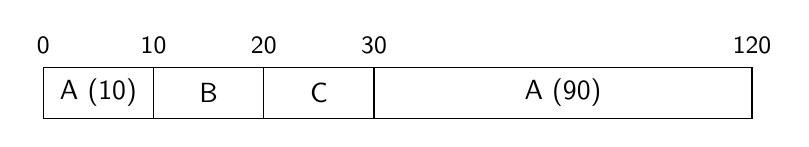
\begin{tikzpicture}
				% Tacche temporali
				\node[font=\sffamily\small] at (0, 0.28) {0};
				\node[font=\sffamily\small] at (1.4, 0.28) {10};
				\node[font=\sffamily\small] at (2.8, 0.28) {20};
				\node[font=\sffamily\small] at (4.2, 0.28) {30};
				\node[font=\sffamily\small] at (9.0, 0.28) {120};
				
				% Blocchi di esecuzione dei Job con prelazione (A interrotto da B e C)
				\draw[fill=white] (0, -0.65) rectangle (1.4, 0) node[midway, font=\sffamily\normalsize] {A (10)};
				\draw[fill=white] (1.4, -0.65) rectangle (2.8, 0) node[midway, font=\sffamily\normalsize] {B};
				\draw[fill=white] (2.8, -0.65) rectangle (4.2, 0) node[midway, font=\sffamily\normalsize] {C};
				\draw[fill=white] (4.2, -0.65) rectangle (9.0, 0) node[midway, font=\sffamily\normalsize] {A (90)};
			\end{tikzpicture}%
		}
	\end{figure}
	Andiamo ad illustrare nel dettaglio cosa accade:
	\begin{enumerate}
		\item Al tempo $t=0$ è presente solo il processo $A$, dunque viene eseguito lui.
		
		\item Al tempo $t=10$ arrivano i processi $B$ e $C$, entrambi della durata di $10s$.
		\begin{itemize}
			\item Essendo arrivato un nuovo processo, viene comparato il tempo di esecuzione rimanente di $A (100-10 = 90s)$ con la durata del processo entrante $10s$.
			
			\item Siccome il processo entrante è più corto, viene subito mandato in esecuzione.
		\end{itemize}
	\end{enumerate}
	Andiamo allora a vedere se è effettivamente migliorato qualcosa, a livello di tempi di completamento:
	\begin{itemize}
		\item $A$ arriva a $t=0$ e finisce a $t = 120$. Tempo di completamento = $120-0=120s$.
		
		\item $B$ arriva a $t=10$ e finisce a $t = 20$. Tempo di completamento = $20-10=10s$.
		
		\item $C$ arriva a $t=10$ e finisce a $t = 30$. Tempo di completamento = $30-10=20s$.
	\end{itemize}
	La media tra queste grandezze è $\frac{120+10+20}{3} = 50s$. Decisamente un miglioramento pensando ai $103.3s$ precedenti.
	
	\begin{osservazione}{Utilità del STFC}{}
		L'algoritmo STCF è \textbf{ottimale} quando si devono \textbf{eseguire processi di cui si conosce la lunghezza} ma che \textbf{possono arrivare in momenti diversi}.
	\end{osservazione}
	
	Tuttavia, anche questo algoritmo non è sicuramente esente da difetti. Immaginiamo una situazione in cui il processo $A$ di durata $100s$ inizia ad essere eseguito a tempo $t=0$. Supponiamo che poi ogni 10 secondi arrivi un processo di durata inferiore ad $A$: verrebbe data priorità a lui, in quanto più corto. A lungo andare verrebbero eseguiti sempre processi di breve durata, ma quello più lungo rimarrebbe in coda ad attendere. Tale situazione è detta \textbf{Starvation}, che è un problema di \textbf{equità}.
	
	\section{Round Robin (RR)}
	Supponiamo di star eseguendo un processo su un sistema multiutente. L'utente A sta modificando un file di testo e l'utente B sta compilando un programma.\\
	Supponendo che la compilazione richieda $10s$, gli algoritmi SJB e STCF darebbero la precedenza a questo processo. Ciò vuol dire però che all'utente A in quei $10s$ verranno ignorate le pressioni di tasti. Ci rendiamo conto di come, in una situazione reale, tali algoritmi non siano molto efficienti.
	\smallbreak
	Ecco perché introduciamo l'algoritmo \textbf{Round Robin (RR)}, che si occupa di schedulare i processi seguendo un loop circolare:
	\begin{itemize}
		\item Anziché eseguire un processo fino alla fine, lo esegue per un breve lasso di tempo.
		
		\item Alla fine di questo lasso di tempo, il processo viene spostato alla fine della coda.
		
		\item Viene eseguito il processo attualmente in testa, e così via finché i processi non sono esauriti...
	\end{itemize}
	Il lasso di tempo entro il cui un processo viene eseguito è detto \textbf{Time Slice} o \textbf{Scheduling Quantum}, il quale deve rispettare le seguenti caratteristiche:
	\begin{itemize}
		\item Deve essere abbastanza lungo da ammortizzare i costi del context switch.
		
		\item Deve essere abbastanza corto da creare l'illusione dell'esecuzione simultanea.
	\end{itemize}
	
	\newpage
	Vediamo un esempio pratico, come fatto prima per i precedenti algoritmi: supponiamo di avere i processi $A, B, C$, tutti che arrivano a $t=0$ e dalla durata di $10s$ ciascuno; il time-slice è impostato a $2s$.
	\begin{figure}[htbp]
		\centering
		\resizebox{0.70\linewidth}{!}{%
			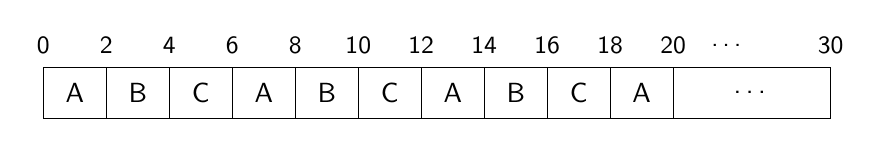
\begin{tikzpicture}
				% Tacche temporali
				\node[font=\sffamily\small] at (0, 0.28) {0};
				\node[font=\sffamily\small] at (0.8, 0.28) {2};
				\node[font=\sffamily\small] at (1.6, 0.28) {4};
				\node[font=\sffamily\small] at (2.4, 0.28) {6};
				\node[font=\sffamily\small] at (3.2, 0.28) {8};
				\node[font=\sffamily\small] at (4.0, 0.28) {10};
				\node[font=\sffamily\small] at (4.8, 0.28) {12};
				\node[font=\sffamily\small] at (5.6, 0.28) {14};
				\node[font=\sffamily\small] at (6.4, 0.28) {16};
				\node[font=\sffamily\small] at (7.2, 0.28) {18};
				\node[font=\sffamily\small] at (8.0, 0.28) {20};
				\node[font=\sffamily\small] at (8.7, 0.28) {\dots};
				\node[font=\sffamily\small] at (10.0, 0.28) {30};
				
				% Blocchi di esecuzione dei Job (Round Robin con quanto = 2)
				\draw[fill=white] (0, -0.65) rectangle (0.8, 0) node[midway, font=\sffamily\normalsize] {A};
				\draw[fill=white] (0.8, -0.65) rectangle (1.6, 0) node[midway, font=\sffamily\normalsize] {B};
				\draw[fill=white] (1.6, -0.65) rectangle (2.4, 0) node[midway, font=\sffamily\normalsize] {C};
				\draw[fill=white] (2.4, -0.65) rectangle (3.2, 0) node[midway, font=\sffamily\normalsize] {A};
				\draw[fill=white] (3.2, -0.65) rectangle (4.0, 0) node[midway, font=\sffamily\normalsize] {B};
				\draw[fill=white] (4.0, -0.65) rectangle (4.8, 0) node[midway, font=\sffamily\normalsize] {C};
				\draw[fill=white] (4.8, -0.65) rectangle (5.6, 0) node[midway, font=\sffamily\normalsize] {A};
				\draw[fill=white] (5.6, -0.65) rectangle (6.4, 0) node[midway, font=\sffamily\normalsize] {B};
				\draw[fill=white] (6.4, -0.65) rectangle (7.2, 0) node[midway, font=\sffamily\normalsize] {C};
				\draw[fill=white] (7.2, -0.65) rectangle (8.0, 0) node[midway, font=\sffamily\normalsize] {A};
				\draw[fill=white] (8.0, -0.65) rectangle (10.0, 0) node[midway, font=\sffamily\normalsize] {\dots};
			\end{tikzpicture}%
		}
	\end{figure}
	Stavolta andiamo a calcolare i \textbf{tempi di risposta} (che ricordiamo essere la differenza tra quando un processo arriva in coda e quando viene eseguito per la prima volta).
	\begin{itemize}
		\item $A$ arriva a $t = 0$ e viene eseguito per la prima volta a $t = 0$. Tempo di risposta $0-0=0s$.
		
		\item $B$ arriva a $t = 0$ e viene eseguito per la prima volta a $t = 2$. Tempo di risposta $2-0=2s$.
		
		\item $C$ arriva a $t = 0$ e viene eseguito per la prima volta a $t = 4$. Tempo di risposta $4-0=4s$.
	\end{itemize}
	Otteniamo come il tempo medio di risposta sia $\frac{0+2+4}{3} = 2s$, il che è un tempo di attesa \textbf{significativamente basso}. Il lettore può provare da solo a calcolare tale grandezza in riferimento ad un algoritmo come SJF.
	
	\begin{osservazione}{Utilità del Round Robin}{}
		Come abbiamo visto, l'algoritmo Round Robin è \textbf{ottimale} per \textbf{minimizzare i tempi di risposta} (cioè per garantire che i processi vengano tutti "serviti" in un tempo ragionevole), tuttavia risulta terribile per quanto riguarda il tempo di completamento.
		\smallbreak
		Considerando sempre l'esempio precedente, abbiamo che $A$ termina a $t=26$, $B$ termina a $t=28$, $C$ termina a $t=30$. Vediamo come il tempo di completamento minimo sia di $\frac{26+28+30}{3} = 28s$, il che è un tempo anche peggiore degli algoritmi SFJ e STCF.
	\end{osservazione}
	
	Possiamo dunque fare una considerazione generale per quanto riguarda i tempi di risposta e di completamento.
	\begin{osservazione}{Trade-off tra risposta e completamento}{}
		\begin{itemize}
			\item Ogni politica che \textbf{ottimizza il tempo di risposta avrà un downgrade sul tempo di completamento}.
			
			\item Ogni politica che \textbf{ottimizza il tempo di completamento avrà un downgrade sul tempo di risposta}.
		\end{itemize}
	\end{osservazione}
	
	\section{Incorporazione dell'I/O}
	Purtroppo, è arrivato anche il momento di rilassare la quarta assunzione, riguardante l'assenza di operazioni di I/O da completare, anche perché queste sono molto più frequenti di quanto ci si possa immaginare.\\
	Come sappiamo avendo studiato gli stati di un processo, quando il job deve svolgere un'operazione di I/O si deve:
	\begin{enumerate}
		\item Mettere il processo in stato \texttt{BLOCKED}.
		
		\item Attendere che l'operazione sia completata, e intanto eseguire altri processi.
		
		\item Una volta completata l'operazione, il processo viene rimesso nella coda dei processi \texttt{READY}.
	\end{enumerate}
	Il punto di un buono scheduler è proprio garantire che venga eseguito un altro processo nel frattempo che il corrente è impegnato in un'operazione di I/O.\\
	La sezione di tempo in cui un processo viene eseguito è detta \textbf{CPU Burst}, mentre quella in cui il processo attende l'I/O si chiama \textbf{I/O Wait}.
	\smallbreak
	
	Tutto bello ma...come lo implementiamo nei nostri algoritmi di scheduling?\\
	Il trucco è trattare ogni CPU Burst come un sotto-processo indipendente, che viene eseguito e schedulato per conto suo.
	\begin{itemize}
		\item Se il processo A ha bisogno di un totale di 50ms di CPU, dividiamo questo tempo in 5 CPU Burst ognuno da 10ms, separati ognuno da operazioni di I/O.
		
		\item Ogni CPU Burst da 10ms viene schedulato come se fosse un processo indipendente.
	\end{itemize}
	
	Vediamo un esempio di questa implementazione con l'algoritmo STCF, con il seguente esempio:
	\begin{itemize}
		\item Il processo A ha 10ms di CPU Burst e 10ms di I/O wait (il tutto ripetuto per 5 volte).
		
		\item Il processo B ha 50ms di solo CPU Burst.
	\end{itemize}
	
	\begin{figure}[htbp]
		\centering
		\resizebox{0.70\linewidth}{!}{%
			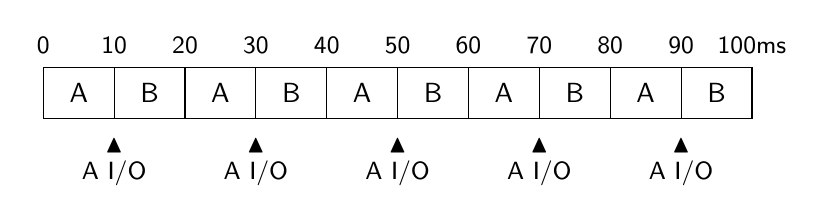
\begin{tikzpicture}
				% Tacche temporali
				\node[font=\sffamily\small] at (0, 0.28) {0};
				\node[font=\sffamily\small] at (0.9, 0.28) {10};
				\node[font=\sffamily\small] at (1.8, 0.28) {20};
				\node[font=\sffamily\small] at (2.7, 0.28) {30};
				\node[font=\sffamily\small] at (3.6, 0.28) {40};
				\node[font=\sffamily\small] at (4.5, 0.28) {50};
				\node[font=\sffamily\small] at (5.4, 0.28) {60};
				\node[font=\sffamily\small] at (6.3, 0.28) {70};
				\node[font=\sffamily\small] at (7.2, 0.28) {80};
				\node[font=\sffamily\small] at (8.1, 0.28) {90};
				\node[font=\sffamily\small] at (9.0, 0.28) {100ms};
				
				% Blocchi di esecuzione dei Job A e B
				\draw[fill=white] (0, -0.65) rectangle (0.9, 0) node[midway, font=\sffamily\normalsize] {A};
				\draw[fill=white] (0.9, -0.65) rectangle (1.8, 0) node[midway, font=\sffamily\normalsize] {B};
				\draw[fill=white] (1.8, -0.65) rectangle (2.7, 0) node[midway, font=\sffamily\normalsize] {A};
				\draw[fill=white] (2.7, -0.65) rectangle (3.6, 0) node[midway, font=\sffamily\normalsize] {B};
				\draw[fill=white] (3.6, -0.65) rectangle (4.5, 0) node[midway, font=\sffamily\normalsize] {A};
				\draw[fill=white] (4.5, -0.65) rectangle (5.4, 0) node[midway, font=\sffamily\normalsize] {B};
				\draw[fill=white] (5.4, -0.65) rectangle (6.3, 0) node[midway, font=\sffamily\normalsize] {A};
				\draw[fill=white] (6.3, -0.65) rectangle (7.2, 0) node[midway, font=\sffamily\normalsize] {B};
				\draw[fill=white] (7.2, -0.65) rectangle (8.1, 0) node[midway, font=\sffamily\normalsize] {A};
				\draw[fill=white] (8.1, -0.65) rectangle (9.0, 0) node[midway, font=\sffamily\normalsize] {B};
				
				% Frecce e indicazioni di I/O per il job A
				\node[font=\sffamily\small] at (0.9, -1.0) {$\blacktriangle$};
				\node[font=\sffamily\small] at (0.9, -1.35) {A I/O};
				
				\node[font=\sffamily\small] at (2.7, -1.0) {$\blacktriangle$};
				\node[font=\sffamily\small] at (2.7, -1.35) {A I/O};
				
				\node[font=\sffamily\small] at (4.5, -1.0) {$\blacktriangle$};
				\node[font=\sffamily\small] at (4.5, -1.35) {A I/O};
				
				\node[font=\sffamily\small] at (6.3, -1.0) {$\blacktriangle$};
				\node[font=\sffamily\small] at (6.3, -1.35) {A I/O};
				
				\node[font=\sffamily\small] at (8.1, -1.0) {$\blacktriangle$};
				\node[font=\sffamily\small] at (8.1, -1.35) {A I/O};
			\end{tikzpicture}%
		}
	\end{figure}
	Ricordiamo che l'algoritmo di scheduling è il STCF, dunque il workflow è il seguente:
	\begin{enumerate}
		\item Il processo A viene schedulato per primo perché la sua durata (10ms, ricordiamo che A è stato suddiviso in sotto-processi indipendenti) è inferiore a quella del processo B (50ms).
		
		\item Dopo 10ms, il processo A entra in I/O Wait per 10ms, tempo durante il quale verrà eseguito il processo B.
		
		\item Avanti così finché uno dei due processi non termina...
	\end{enumerate}
	
\end{document}